\clearpage
\section[Une plate-forme d'exploration de données de simulations : SimEDB]{Une plate-forme d'exploration de données de simulations : SimEDB%
\sectionmark{SimEDB}}\label{sec:SimEDB}

La \cref{sec:explorer-sorties-simfeodal} (\cnameref{sec:explorer-sorties-simfeodal}) a décrit les étapes successives d'avancement dans l'exploration des données en sortie de SimFeodal, depuis l'observation en direct des simulations (\og pré-filtrage\fg{}) jusqu'au besoin d'une plate-forme permettant l'exploration et la comparaison interactive des sorties de simulation.
La plate-forme proposée en réponse à ce besoin, SimEDB\footnote{
\textbf{Sim}Feodal \textbf{E}xploration \textbf{D}ash\textbf{B}oard, voir la note de bas de page \ref{ftn:origine-simedb}, \cpageref{par:introduction-nom-simedb}.
}, dans un objectif de généricité et d'adéquation, se devait aussi de répondre à de nombreuses contraintes, aussi bien liées aux possibilités offertes qu'à l'usage qui en serait fait.
Dans cette partie, nous nous attacherons donc à présenter les contraintes qui ont guidé la conception de SimEDB, ainsi que les choix, méthodologiques et techniques, qui en ont résulté.\vspace{-0.5cm}

\subsection{Contraintes}

\subsubsection{Adapter la complexité aux utilisateurs}

Dans le domaine de l'Interface Homme-Machine (IHM), il est courant de considérer qu'un outil d'analyse et de représentation doit être adapté à un public.
La \cref{fig:cartography3}, emblématique de la conception de géovisualisations par Alan \textsc{MacEachren}, replace ainsi les types d'usage d'une plate-forme d'exploration selon trois axes : le niveau d'expertise des utilisateurs visés (\textit{users}), le niveau d'interaction souhaité (\textit{interaction}) et l'objectif poursuivi par la (géo)visu\-alisation (\textit{task}).
D'après l'auteur, à un niveau d'expertise de l'utilisateur correspond un unique degré d'interaction et un unique objectif : dans le cube, seule une \og droite\fg{} des usages possibles est présente.
L'auteur décompose ces usages en quatre types :
\begin{itemize}
	\item Pour le grand public (\textit{users} de type \textit{public}), l'objectif est de transmettre une information simple (\textit{info sharing}). Le niveau d'interaction avec la géovisualisation doit donc être faible. Il s'agit d'une tâche de présentation (\textit{present}).
	\item Pour un public légèrement plus connaisseur, on peut augmenter le niveau d'interaction. On entre alors dans un but de synthèse (\textit{synthesize}).
	\item En ciblant un niveau encore supérieur d'expertise chez l'utilisateur, et en visant à de la construction de connaissance plus qu'à une transmission de connaissance, on augmente encore le niveau d'interaction.
	La géovisualisation a alors pour but l'analyse (\textit{analyze}).
	\item Au plus haut niveau d'interaction, d'expertise et de recherche, la géovisualisation peut servir d'outil d'exploration (\textit{explore}).
\end{itemize}

%\begin{figure}[H]
%\hspace*{\fill}%
%\begin{minipage}[t]{.46\linewidth}
%\centering
%\captionsetup{width=.9\linewidth}
%\vspace{0pt}
%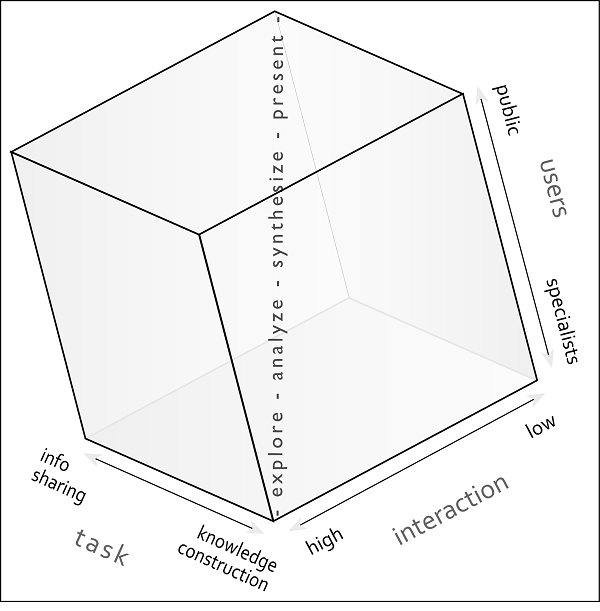
\includegraphics[width=\linewidth]{img/CV35-Fig2a-600.png}
%\caption{\og \textit{An update to Cartography³, 10 years after its conception}\fg{}, par \cite{coltekin_geovisualization_2018}, d'après \cite[10]{maceachren_geovisualization_2004}.}
%\label{fig:cartography3}
%\end{minipage} \hfill
%\begin{minipage}[t]{.46\linewidth}
%\centering
%\captionsetup{width=.9\linewidth}
%\vspace{0pt}
%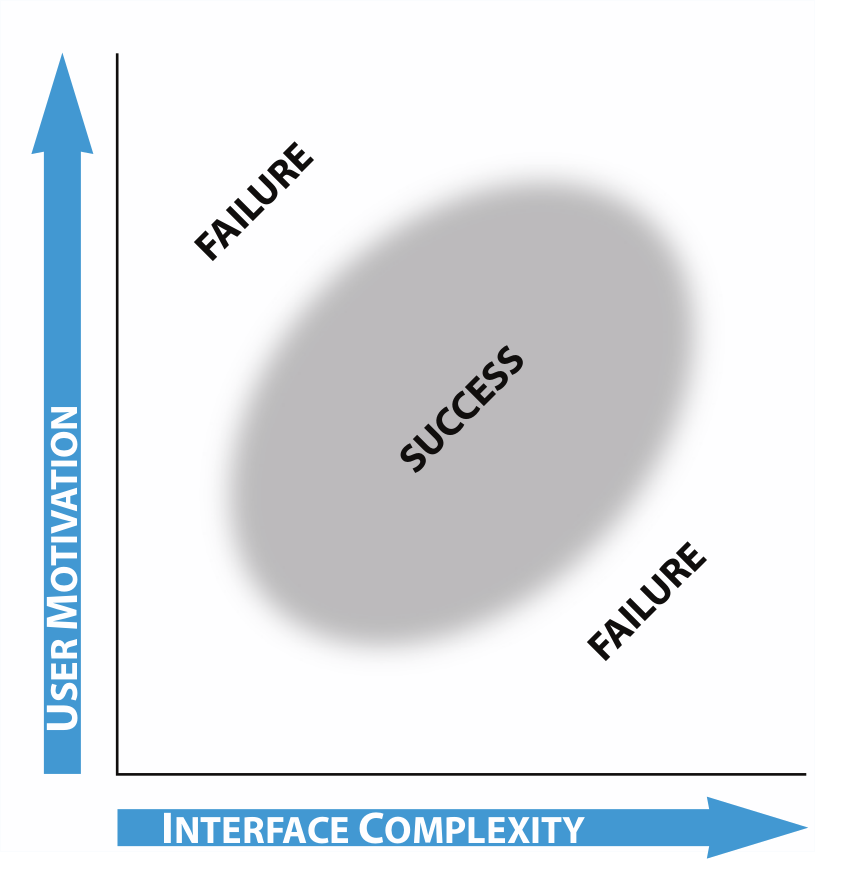
\includegraphics[width=\linewidth]{img/Roth_Interface_Complexity.png}
%\caption{\og \textit{Interface complexity versus user motivation. }\fg{}, \cite[79]{roth_interactive_2013}.}
%\label{fig:interface-complexity}
%\end{minipage}
%\medskip
%\end{figure}

\begin{figure}[H]
\centering
\vspace{0pt}
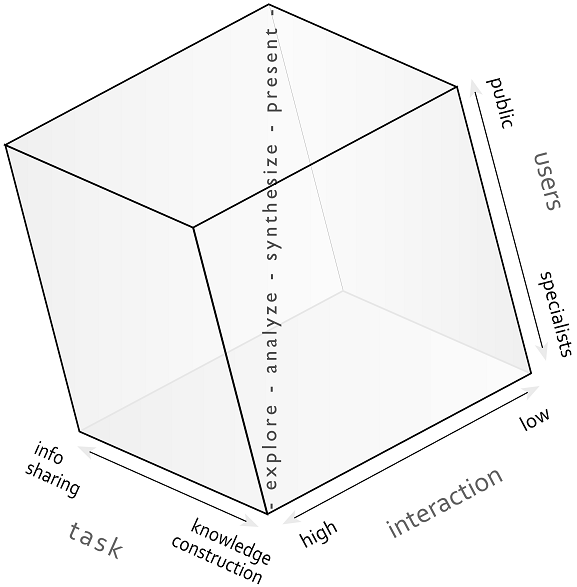
\includegraphics[width=.7\linewidth]{img/cartography3.png}
\captionsetup{width=.7\linewidth}
\caption{\og \textit{An update to Cartography³, 10 years after its conception}\fg{}, par \cite{coltekin_geovisualization_2018}, d'après \cite[10]{maceachren_geovisualization_2004}.}
\label{fig:cartography3}
\end{figure}

\textcite[16]{roth_interactivity_2015} commente cette figure en effectuant une assimilation entre niveau d'interaction et complexité de l'interface de l'outil de géovisualisation : \og All participants agreed that user expertise requires increased interface complexity, as suggested by the Cartography³ framework\fg{}.

La plateforme SimEDB est conçue pour être utilisée par des experts thématiques (l'équipe de modélisation de SimFeodal), avec un objectif clairement inscrit dans la construction de connaissance.
A ce titre, et d'après \textsc{MacEachren}, le niveau d'interaction avec l'outil de géovisualisation devrait être élevé (forte complexité de l'interface pour \textsc{Roth}) et ancrer l'usage dans une dimension exploratoire.



\paragraph*{Des utilisateurs hétérogènes mais captifs}

SimEDB est pourtant pensé à un niveau intermédiaire, entre l'analyse et la synthèse, dans le cube de la \cref{fig:cartography3}.
Il ne s'agit ainsi pas d'explorer des données, au sens de MacEachren, qui sous-entend par cette exploration (\textit{explore}) la recherche d'informations dans un jeu de données inconnu de l'utilisateur.
Le besoin identifié consiste à permettre aux utilisateurs d'explorer des sorties de simulation à travers des indicateurs déjà pensés et constitués.
Il ne s'agit pas de proposer un outil d'exploration de données brutes, permettant de créer à la volée des nouveaux indicateurs, via une approche d'exploration \og naïve\fg{}.
Au contraire, l'exploration est guidée par les indicateurs, et la tâche s'apparente plus à de l'analyse de résultats de simulations, voire à de la synthèse des spécificités des résultats issus d'expériences différentes.
L'objectif de SimEDB s'écarte donc du \og modèle\fg{} de \textsc{MacEachren}, puisqu'il ne se situe pas sur la \og droite\fg{} des usages (voir la \cref{fig:cartography3-simedb}).

\begin{figure}[H]
\hspace*{\fill}%
\begin{minipage}[t]{.46\linewidth}
\centering
\captionsetup{width=.9\linewidth}
\vspace{0pt}
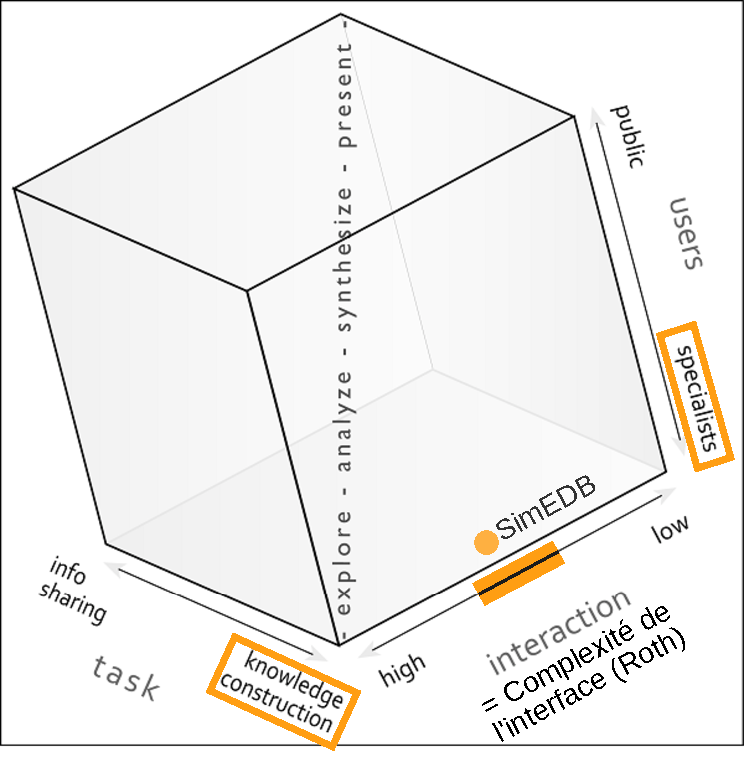
\includegraphics[width=\linewidth]{img/Cartography3_SimEDB.pdf}
\caption{Positionnement de SimEDB dans le cube \textit{Cartography³} de \textsc{MacEachren}.}
\label{fig:cartography3-simedb}
\end{minipage} \hfill
\begin{minipage}[t]{.46\linewidth}
\centering
\captionsetup{width=.9\linewidth}
\vspace{0pt}
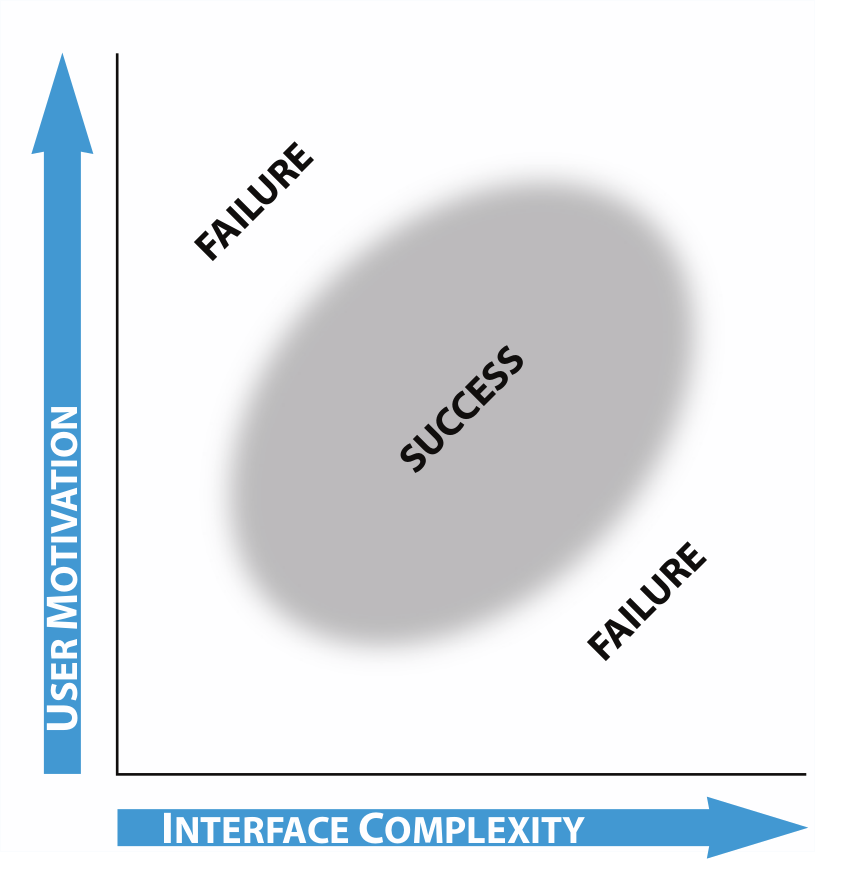
\includegraphics[width=\linewidth]{img/Roth_Interface_Complexity.png}
\caption{\og \textit{Interface complexity versus user motivation. }\fg{}, \cite[79]{roth_interactive_2013}.}
\label{fig:interface-complexity}
\end{minipage}
\medskip
\end{figure}

Cet écart au modèle conceptuel de MacEachren s'explique notamment par la diversité des utilisateurs de SimEDB.
Il serait absurde de qualifier un niveau d'expertise général des utilisateurs tant les spécificités de cette expertise sont nombreuses.
Entre des profils de spécialiste thématiciens, de modélisateurs ou encore de géomaticiens, l'expertise est présente, mais concernant des champs différents, toutefois tous intéressés par l'exploration des sorties de SimFeodal.

Il est dès lors peu évident de se fixer sur un degré de complexité à atteindre dans la plate-forme d'exploration : un niveau faible serait frustrant pour les utilisateurs avancés, et un niveau avancé serait source de confusion et donc de perte de motivation pour les utilisateurs moins expérimentés (\cref{fig:interface-complexity}).

Une spécificité du cas d'usage de SimEDB permet toutefois de miser sur une bonne motivation générale des utilisateurs, et donc sur la possibilité de créer un outil à l'interaction plus complexe qu'un simple présentoir de données.
Contrairement à une utilisation grand public, qui ne présente aucun engagement vis-à-vis d'une interface d'exploration de données, ou à l'inverse contrairement à des domaines experts où chaque utilisateur dispose de ses propres outils et méthodes pour explorer un jeu de données, le public cible de SimEDB est \og captif\fg{}.
On entend par là que les utilisateurs concernés par SimEDB ne disposent pas d'autre solution que de passer par cette plate-forme pour explorer les données issues de sortie de simulation, en particulier en raison des contraintes liées aux caractéristiques de ces données (leur masse par exemple, voir la \cref{subsec:donnees-indicateurs}, \cnameref{subsec:donnees-indicateurs}).
On peut dès lors se permettre de développer une interface plus complexe que si l'on visait un plus large public.

\paragraph*{Intuititivé de l'usage au regard des applications traditionnelles}

En dépit de cette motivation, les utilisateurs de SimEDB demeurent majoritairement des experts thématiciens, potentiellement peu familiarisés à l'exploration de données interactives.
Afin que le temps d'exploration des données issues de SimFeodal soit dévoué à la compréhension et à la synthèse de ces données plutôt qu'à un apprentissage ou amélioration en exploration de données, il a été choisi de créer une application aussi simple que possible au regard des fonctionnalités principales qu'elle devait permettre : observer les indicateurs de sortie de simulation pour des expériences données, et les comparer entre elles aussi efficacement que possible.

Il n'était donc pas question de construire un nouveau \og logiciel expert \fg{}, doté de dizaines de fonctionnalités avancées, mais au contraire, de simplifier au maximum l'interface pour ne pas encombrer et complexifier l'utilisation de ces fonctionnalités principales.

On souhaitait une plate-forme aussi épurée que possible, plutôt que de partir, par exemple, sur la personnalisation et l'adaptation de l'un des outils d'exploration existants et dédiés à offrir une forte possibilité de manipulation\footnote{
\colorbox{Cyan}{Lena : \og Éventuellement dire pourquoi recherche de généricité dans un créneau bien spécifique ?}
}.


\subsubsection{Efficacité}

Dans la description du choix du SGBD, on a mentionné une première fois l'intérêt de disposer d'une solution d'interrogation de données qui garantisse une certaine rapidité dans l'exécution des requêtes.
Sans entrer dans le détail des recherches en IHM, on peut compléter ce besoin de rapidité par deux aspects complémentaires.
Une solution interactive qui minimise les latences permet (1) de motiver l'utilisateur, c'est-à-dire de ne pas le décourager d'utiliser l'application, et (2) de lui faire conserver sa concentration\footnote{
Avant de spécifier ce sujet, notons que quand le délai entre une interaction avec un outil informatique et le retour qu'il doit produire (affichage de graphique par exemple) est important, l'utilisateur perd en capacité d'association entre son action et le retour observé.
Typiquement, dans un processus d'exploration de données, plus ce délai est faible, plus l'utilisateur peut mobiliser son intuition pour évaluer, par exemple, les relations entre des variables ou des individus.
} (\textit{focus}).

Le premier point a été abordé plus haut (\cref{subsubsec:interroger-robuste-efficace}), et surtout, en raison de la \og captivité\fg{} de l'utilisateur évoquée ci-dessus, ne s'applique que marginalement à notre cas d'étude.
Des délais trop importants pourraient décourager l'utilisateur, mais en l'absence d'alternative pour explorer les sorties de simulation, cela n'a pas un impact trop important.

\paragraph*{Conserver la concentration}

Le problème de la concentration de l'utilisateur demeure, lui, critique.
Des études ont montré, depuis longtemps \autocite{mackenzie_lag_1993}, qu'il y avait un lien fort entre la performance d'une interrogation visuelle et le délai nécessaire à son obtention.
\cite[8]{liu_effects_2014} montrent ainsi qu'avec un simple délai de 500 millisecondes (ms), la qualité des observations, des généralisations qui peuvent être tirées des données, et des hypothèses émises, décroît nettement chez l'utilisateur.
Les auteurs indiquent d'ailleurs que cette diminution est plus importante encore quand l'exploration est effectuée par des actions de \textit{brushing} et de sélections croisées (\textit{linking}), deux méthodes qui sont au cœur de SimEDB : \og For example, more aggressive caching or prefetching methods may be employed for operations sensitive to small variations in latency, such as brushing and linking \fg{} \autocite[9]{liu_effects_2014}.

\cite{forch_are_2017}, pour leur part, étudient la perception du délai de réponse lors d'interactions menées avec une souris d'ordinateur.
Ils concluent ainsi que les utilisateurs perçoivent des délais d'attente inférieurs à 100 ms, mais notent que les utilisateurs n'en sont pas pour autant perturbés, en particulier ceux qui ont le moins l'habitude de réactions rapides\footnote{
Ils remarquent ainsi que les utilisateurs plus habitués à des jeux vidéos rapides (\og highly dynamic computer games, such as action games, racing games, or first person shooter games [...]\fg{}, \cite[51]{forch_are_2017}) sont plus vite affectés par le délai de réponse que les autres.
}.

Concernant le champ, plus spécifique, des \textit{visual analytics}, nous n'avons pas trouvé d'articles de référence permettant d'établir une comparaison de l'efficacité des résultats trouvés selon la latence de la réponse.
Les auteurs de ce champ recommandent de prêter attention à la rapidité de rendu et à son optimisation, mais sans que ne trouvions de résultats plus précis :
\begin{quotation}
\noindent \og
When simple pattern finding is needed, the importance of having a fast, highly interactive interface cannot be emphasized	enough.
If a navigation technique is slow, then the cognitive costs can be much greater than just the amount of time lost, because an entire train of thought can become disrupted by the loss of the contents of both visual and nonvisual working memories.
\fg{}\\
\mbox{}~ \hfill  \cite{ware_information_2012}, tiré de \cite[12]{amirpour_amraii_human-data_2018}.
\end{quotation}

Tout au plus pouvons-nous émettre l'idée qu'il serait évident que la latence acceptée dans un environnement graphique de ce type soit largement supérieure à celle des environnements virtuels (réalité augmentée, visualisations immersives\ldots), sans pour autant que nous ne puissions quantifier cet écart.
On peut tout de même s'appuyer sur une estimation du temps de concentration, lié à la mémoire à court terme, décrit par \citeauteur{shneiderman_designing_2004} :
\begin{quotation}
 	\noindent\og
 	A central issue is the limitation of short-term memory capacity, as outlined in George Miller's (1956) classic paper, ``The magical number seven, plus or minus two.''
 	Miller identified the limited capacities people have for absorbing information.
 	People can rapidly recognize approximately 7 (this value was contested by later researchers, but it serves as a good estimate) chunks of information at a time and can hold those chunks in short-term memory for 15 to 30 seconds.
 	The size of a chunk of information depends on the person's familiarity with the material.
	\fg{}\\
	\mbox{}~ \hfill  \cite[459]{shneiderman_designing_2004}.
\end{quotation}

Si l'on considère qu'un indicateur contient à peu près ces sept \og morceaux d'information\fg{}\footnote{
Par exemple, pour un indicateur simple tel que l'évolution du nombre de foyers paysans isolés au cours du temps, il faut retenir le niveau initial, le niveau final, la tendance de sa courbe et éventuellement les dates des deux ou trois inflexions ou décrochages que l'on peut y constater.
} et que l'on se place dans une phase de comparaison entre les résultats de sortie de simulation de deux expériences différentes, il faut alors que le temps de sélection graphique de la seconde expérience et d'affichage de l'indicateur correspondant soit inférieur à quinze secondes.
En prenant en compte le temps de sélection graphique, qui peut demander une manipulation de l'interface de l'application (voir \cref{par:simedb-resize-parcoords} et \cref{fig:resizing}, p.~\pageref{fig:resizing}), cela implique qu'un indicateur doit être généré en un maximum de 5 secondes\footnote{
	En comptant 10 secondes pour la sélection de l'expérience.
	On prend ici le cas extrême (faible durée de concentration et manipulation longue), afin de garantir une expérience utilisateur satisfaisante quelque soit l'état de concentration de l'utilisateur.
}.

Selon ces différentes considérations, dans le cadre de SimEDB, on doit donc viser à développer une plate-forme aussi rapide que possible.
Celle-ci doit donc viser des temps de latence maximale de l'ordre de quelques secondes maximum, tout en sachant, dès le départ, qu'il sera impossible d'arriver aux délais de 100 ms ou 500 ms évoqués précédemment, ne serait-ce que parce que le temps de requête des données -- sans compter le temps de rendu graphique -- est déjà supérieur d'un ordre de grandeur.

\subsubsection{Interopérabilité et évolutivité}

Une autre contrainte forte tient cette fois au choix de l'environnement informatique qui accueillera la plate-forme d'exploration.
On peut résumer ce choix à deux alternatives : un environnement local, en installant l'application sur l'ordinateur de chaque utilisateur, ou un environnement distant, où l'application serait donc accessible à distance, par exemple via une interface web\footnote{
Cette question était également posé pour le choix du SGBD en \cref{par:stockage-centralise}.
L'outil d'exploration et l'architecture de données sont cependant indépendants, et le choix d'un stockage des données sur un serveur distant n'implique aucunement que l'application suive la même logique.
On peut ainsi avoir un SGBD distant qui serait interrogé par une application locale.
}.
Ce choix a des nombreuses répercussions, aussi bien en matière de possibilité d'accès que de facilité à faire évoluer la plate-forme.

Le choix le plus classique est de développer une application installable sur un ordinateur : cela permet de garantir une utilisation à tout moment, sans contrainte d'accès au réseau internet.
Cela permet aussi d'obtenir de meilleurs performances, puisque la rapidité de l'application dépend à ce moment uniquement de la puissance de l'ordinateur, plutôt que de devoir souffrir du passage par l'intermédiaire d'un serveur.

Comme pour le choix du type de SGBD, nous avons cependant préféré nous orienter sur une solution de type distante, pour des raisons d'interopérabilité et d'évolutivité que nous allons décrivons ici.


\paragraph*{Différents supports d'interrogation}
La performance d'une application locale, par rapport à une application distante, est un atout extrêmement intéressant, comme on vient de le montrer plus haut.
Pourtant, cela implique une énorme contrainte : l'application doit être interopérable entre les différents systèmes d'exploitations (\textit{Operating System}, OS) et versions de ceux-ci.
Les utilisateurs potentiels de SimEDB, représentation fidèle des acteurs de la recherche, se partagent ainsi entre les trois systèmes d'exploitations majoritaires (Windows, MacOs, Linux).

Pour permettre à chacun d'utiliser SimEDB, il faudrait donc que le développement de cette plate-forme soit compatible avec ces différents OS, ce qui est une contrainte considérable en développement logiciel.

Ne mentionnons même pas les nouveaux OS, centrés autour d'usages tactiles, tels qu'on les retrouve sur les tablettes et autres \textit{smartphones}, qui demandent, eux aussi, de nombreuses spécificités de développement.

En somme, disposer d'une application locale universelle, c'est-à-dire utilisable quelque soit le support informatique, est une quasi-impossibilité technique, et un objectif en soit, que notre travail de recherche ne cherche aucunement à résoudre.
Pour garantir la faisabilité d'une plate-forme d'exploration de données locale dédiée aux données de simulation de SimFeodal, il faudrait donc commencer par restreindre son champ d'application à un ou deux supports officiels, par exemple l'OS Windows, abandonnant de fait les utilisateurs potentiels ne disposant pas de cette architecture logicielle.

\paragraph*{Gérer les mises à jours et modifications}

Comme pour les bases de données (\og \cnameref{par:stockage-centralise}\fg{}, \cpageref{par:stockage-centralise}), la question de l'application locale ou distante pose un contrainte supplémentaire en matière de maintenabilité et d'évolutivité de la plate-forme choisie.
Dans le cadre d'une application locale (correspondant au distribué en SGBD), la distribution des différentes mises à jour de l'application entraînent nécessairement l'installation locale, à chaque fois.
Le risque est alors que tous les utilisateurs ne disposent pas d'une même version, ce qui peut entraîner, par exemple, des contradictions dans l'évaluation d'expériences, certains utilisateurs ayant accès à une version proposant des différences dans la manière de calculer ou d'afficher les indicateurs.

Sans aller jusqu'à ces extrêmes, notons qu'avec une application locale, le temps de répercussion d'une modification du code de la plate-forme est plus important : il faut en effet réinstaller sur chaque poste le logiciel ainsi modifié.
Cela disqualifie de fait des modifications \og en direct\fg{}, par exemple lors d'une session collective d'exploration des résultats où les utilisateurs auraient des propositions de modifications à faire, ne serait-ce que pour des changements aussi infimes que des titres de graphiques ou d'axes.

\paragraph*{Le choix d'une application web}

Au contraire, avec une application distante, donc basée sur l'accès, par un navigateur internet, à une application centralisée, ces problèmes ne se posent pas : des navigateurs sont disponibles pour tous les OS existants (OS dédiés aux ordinateurs ou aux usages mobiles), et interprètent de la même manière une page web, indépendamment de leur support de consultation.
De plus, comme pour les SGBD, l'usage d'une plate-forme distante permet une répercussion instantanée des mises à jour et corrections : un utilisateur n'a qu'à rafraichir sa page pour que la dernière version de l'application s'affiche.
De la même manière, si un utilisateur souhaite étudier un nouvel indicateur, non prévu auparavant, le temps de déploiement peut être suffisamment court pour que cela soit possible au cours d'une même session d'exploration de données.

Il y a toutefois un désavantage vis-à-vis de solutions entièrement locales, puisque les données permettant l'affichage des indicateurs doivent transiter sur le réseau internet.
En cas de connexion lente, l'usage de l'application sera particulièrement difficile, et même impossible en l'absence d'une connexion.

Cette lenteur relative est toutefois compensée par un avantage de la centralisation de l'application : les calculs, parfois lourds, ne reposent pas sur les capacités individuelles des ordinateurs clients.
En installant l'application sur un serveur dédié, il suffit donc d'augmenter les caractéristiques de celui-ci pour que les performances soient améliorées pour chacun des utilisateurs de l'application.

Dans le cas de SimEDB, nous disposons de ressources informatiques largement suffisantes\footnote{
En nous appuyant dans un premier temps sur un serveur de calcul interne à l'UMR Géographie-cités, puis sur un serveur de calcul partagé mis à disposition par la \href{https://www.huma-num.fr/}{\og Très Grande Infrastructure de Recherche\fg{} Huma-Num} ensuite.
} pour assurer une rapidité de traitement des données et ainsi permettre à l'application SimEDB de se dégager de ce \og goulot d'étranglement\fg{} technique qu'aurait sinon éprouvée la plate-forme.

\subsubsection{Généricité de l'interrogation et indépendance aux données}

La dernière contrainte, plus technique, tient au besoin de généricité d'une plate-forme d'exploration de données vis-à-vis des données qu'elle interroge.
On a résumé les possibilités et choix effectués en matière de SGBD (\cref{subsec:capacite-interrogation} :  \og \cnameref{subsec:capacite-interrogation}\fg{}), et décidé de ne retenir que des SGBD permettant une interrogation standardisée via des connecteurs génériques et un langage universel (le SQL).

L'infrastructure de stockage et d'organisation des données a ainsi été conçue pour être aussi générique que possible.
Encore faut-il que la plate-forme d'exploration de données soit elle aussi aussi générique que possible, et donc en mesure de profiter de l'universalité du SGBD choisi.

\paragraph*{Indépendance au support de données}
Une contrainte forte est donc constituée par la capacité de la plate-forme a être indépendante de la source des données : quelque soit le SGBD choisi, les requêtes émises par la plate-forme doivent être les mêmes, sans requérir d'adaptations spécifiques en dehors de la désignation du lieu de stockage des données	et des pilotes du SGBD.

Dans les faits, lors de la construction de SimEDB (cf. \cref{sec:explorer-sorties-simfeodal} : \og \cnameref{sec:explorer-sorties-simfeodal}\fg{}), plusieurs solutions de stockage de données ont été employées successivement, au fur et à mesure des limites rencontrées chez chacune.
Depuis les premières implémentations des rapports automatiques jusqu'à l'utilisation de SimEDB dans son état actuellement discuté, les données de sorties de simulation ont ainsi été tour à tour interrogées depuis de simples fichiers CSV au départ jusqu'au SGBD ultra-performant MapD, en passant par des solutions intermédiaires plus classiques (SQLite et MonetDB notamment).

Il n'était donc aucunement question d'avoir à adapter le code source des programmes permettant de générer les indicateurs depuis les données, mais au contraire, de s'assurer d'utiliser des bibliothèques logicielles indépendantes des données, c'est-à-dire capables d'exécuter les mêmes chaînes de traitements quelle que soit la provenance des données.

On peut expliciter ce propos à l'aide de l'exemple caricatural des logiciels de type tableurs.
Dans ce type d'application, on peut écrire des programmes (les \og macros\fg{}) qui permettront l'ouverture d'un fichier CSV et effectueront des calculs dessus pour en tirer par exemple des résumés.
Dans ce même tableur, on peut aussi faire appel à des sources de données différentes (bases de données Access ou SQL par exemple), mais les programmes (macros) seront alors à ré-écrire en quasi-totalité pour les adapter aux différences de sources de données.

Dans notre cas, les sources de données ayant très largement évolué au cours du temps, on ne pouvait faire reposer notre application sur une plateforme qui demande une adaptation forte à la provenance des données, comme c'est le cas des tableurs.
Il était donc nécessaire de s'appuyer sur des environnements logiciels (les bibliothèques logicielles) permettant une forte généricité vis-à-vis des sources de données.

\paragraph*{Indépendance aux requêtes et modularité de l'implémentation \label{par:DSL}}

Pour garantir cette généricité, il est donc nécessaire de s'assurer que le mode de communication de la plate-forme vers les données soit bien basé sur un langage universel : le SQL.
Il convient donc de choisir un ensemble de technologies permettant de générer des requêtes SQL, quand bien même l'expression de ces requêtes elles-mêmes serait conçue dans un autre langage.
Pour les requêtes complexes, le SQL tend en effet a être peu lisible, les opérations s'emboîtant les unes dans les autres de manière très linéaires, et donc, souvent verbeuses.
En SQL pur, il est donc peu évident de créer une implémentation modulaire d'une requête, c'est-à-dire permettant une factorisation des commandes et un paramétrage des entrées.

Les indicateurs de sortie de SimFeodal sont, on l'a vu, assez fréquemment basés sur le même type d'opération : on observe par exemple souvent l'évolution du nombre d'agents d'un certain type (agrégats, foyers paysans\ldots)au cours du temps.
Dans le cas de cet exemple, en SQL, pour spécifier une requête permettant de récupérer le nombre de foyers paysans au cours du temps, groupés par année et avec un filtre sur certaines simulations, il ne faut que quelques lignes de code.
Pour que cette requête devienne générique, c'est-à-dire indépendante du type d'agent qui en deviendrait un argument,  il est nécessaire d'y ajouter de nombreuses lignes de code.
Cela revient potentiellement à doubler, pour chacun des indicateurs, la longueur du code-source requis pour l'expression des requêtes, et bien sûr à les rendre plus complexe à modifier et corriger.
De plus, les modes d'expression qui permettent de modulariser du code SQL peuvent varier fortement selon les SGBD choisis, n'étant pas strictement décrits dans les normes SQL.
Par exemple, la déclaration d'une variable, par exemple pour paramétrer le nom de la table contenant les agents, est très différente dans les deux SGBD les plus utilisés (MySQL et PostgreSQL).

Faire appel à un langage intermédiaire, générant du SQL en sortie depuis une entrée sous forme d'un \og \textit{Domain Specific Language}\fg{} (DSL) permet ainsi de bénéficier d'une part de l'universalité du SQL, et d'autre part, d'une syntaxe plus expressive que celle du SQL.
En utilisant un DSL, plus adapté à la manipulation de données qu'à la sélection de sous-ensembles, on gagne donc en modularité d'implémentation , et donc en ré-utilisation de fonctions plus génériques, ce qui permet de disposer d'un code-source plus robuste, ré-utilisable et évolutif.

\subsubsection*{Conclusion : Vers une plate-forme web générique et intuitive}

Dans cette sous-partie, nous avons présenté les principales contraintes qui ont orienté le choix des cadres méthodologiques et techniques utilisables pour concevoir une plateforme telle que SimEDB.

En premier lieu, on fait le choix de se tourner vers une plate-forme implémentée sous forme d'application web, utilisable depuis un simple navigateur -- donc inter-opérable entre les différents supports technologiques --, ce qui exclue de fait quantités d'outils, de logiciels et de bibliothèques logicielles pensées pour l'exploration interactive de données.

On souhaite de plus que la plate-forme utilisée dispose d'une interface aussi épurée que possible, donc nécessairement très adaptée au cas particulier des données issues de simulation que l'on manipule.
Là encore, l'étendue des possibles est restreinte, éliminant l'ensemble de solutions \og clefs-en-main\fg{}, par exemple conçues autour des \og webSIG\fg{} ou de bibliothèques logicielles de visualisations interactives intégrées.

L'utilisation de la plate-forme doit être aussi efficace que possible, en cherchant à minimiser les temps de latence entre sélection interactive et affichage des indicateurs en résultant.
On devra donc privilégier des ensembles technologiques récents et performants, intrinsèquement dédiés à l'interactivité, au détriment de \textit{frameworks} plus génériques.
%, conçus pour une forte diversité d'usage plutôt que pour la tâche très spécifique que constitue la manipulation interactive de données.

Enfin, il faut que cette solution, dans la mesure du possible, soit en mesure de proposer une syntaxes d'interrogation de données modulaire, factorisée, et plus expressive que le SQL sur lequel elle doit toutefois s'appuyer.

Ces contraintes sont des éléments génériques à prendre en compte dans la conception d'un outil d'exploration de données, et elles dépassent largement notre seul cas d'utilisation.
Nous n'avons pour autant pas tenté de brosser un paysage complet des contraintes potentielles, liées aux différents usages possibles, qui peuvent guider les choix techniques et méthodologiques de la conception d'un outil.
La relative spécificité de SimEDB tient à la combinaison des contraintes identifiées et à la combinaison des choix effectuées pour les dépasser, que nous allons maintenant expliciter.

\clearpage
\subsection{Construire une plate-forme interactive pour l'exploration de sorties de simulation}

Dans cette dernière sous-partie, nous allons donc présenter les choix -- techniques, esthétiques et interactifs -- qui ont été adoptés dans la conception et l'implémentation de SimEDB.
Nous les présentons ici de manière linéaire, dans l'ordre quasi-chronologique du développement, mais il est important de garder en considération que ces éléments sont intimement intriqués.
Un choix technique, par exemple, peut conditionner les types d'interactions possibles, parce que l'utilisation de telle méthode d'interaction peut n'être proposée que dans tels et tels environnements logiciels.

Notons enfin que l'application SimEDB présentée ici, aussi bien dans son usage que dans sa conception, représente un instantané de développement, qui correspond à la période de rédaction du présent chapitre :
à l'instar d'un modèle, une plate-forme peut et doit évoluer pour s'adapter aux besoins de ses utilisateurs tant qu'elle est utilisée.
Les technologies et choix esthétiques introduits n'ont pas toujours été présents, et auront sans doute à évoluer dans la suite de la \og durée de vie\fg{} de SimEDB.
Pour les raisons évoquées en termes de facilité de mise à jour d'une solution distante, cela ne pose toutefois aucun problème vis-à-vis de l'utilisation de la plate-forme, largement indépendante, en matière de temporalités, du présent ouvrage.

\subsubsection{Choix des technologies}

Nous présentons ici les technologies mobilisées dans le cadre du développement de SimEDB.
Le but n'est pas d'entrer dans les détails de l'implémentation\footnote{
	Le code source de SimEDB -- et l'historique de son versionnement -- sont, pour cela, disponibles en ligne sous licence libre, sur la plate-forme Github : 
	\faGithub~\href{https://github.com/RCura/SimEDB}{github.com/RCura/SimEDB}
}, mais bien de justifier et présenter les choix relatifs aux technologies employées, en restant à un niveau assez général\footnote{
À ce titre, les quelques lignes de codes présentes par la suite servent un but illustratif et descriptif, et nous semblent remplir ce rôle bien plus efficacement que n'importe quel schéma structurel ne le pourrait.
}.
Il nous paraît important d'entrer dans ces choix qui relèvent plus de la technique que de la méthodologie en ce qu'ils concourent de la volonté de reproductibilité de la thèse, et particulièrement de la reproductibilité de la démarche, conceptuelle et méthodologique, mise en place.
Nous portons la conviction que l'ensemble de technologies assemblées ici dans notre \og chaîne de traitement\fg{} est très largement ré-utilisable, dans le cadre d'adaptations à d'autres cas d'études, mais aussi et surtout, pour une multitude de problématiques requérant une analyse visuelle de données massives (\hl{on y reviendra dans le chap 7}).

\paragraph*{Technologies webs \og natives\fg{}  et adaptativité}

Au cours de la dernière décennie, les interfaces physiques de consultation de médias informatiques se sont largement diversifiées.
Cela a provoqué une hétérogénéisation importante aussi bien des modes d'interaction (dispositifs \og tactiles\fg{}) que des modes d'affichages (les tailles et résolutions des écrans n'ont jamais été aussi diverses et imprévisibles).

En conséquence, les normes de présentations graphiques ont évolué, vers plus d'\og~adaptativité\fg{}, en particulier avec l'avènement du \og responsive web design\fg{} (\og conception de sites web adaptatifs\fg{}) qui permet de prévoir efficacement l'agencement d'une page web quelque soit le support de consultation.

Les technologies qui prédominaient dans la réalisation d'applications web interactives il y a quelques années\footnote{
	Applications en \textsc{Flash},  \textit{applets} Java\ldots
}  ont largement disparu suite à un manque d'adaptation à ces nouveaux support.

Pendant ce temps, de nouveaux standards du développement web (\textsc{HTML5} entre autre) ont émergé et atteint un niveau de maturité suffisant pour remplacer l'ensemble des possibilités (et les étendre) proposées par ces anciens environnements trop monolithiques.

Ces technologies, aujourd'hui indispensables, reposent sur des codes standardisés, verbeux et peu explicites\footnote{
	Il suffit de consulter le code-source d'une page web contenant des visualisation interactives pour le constater.
	Les assemblages de langages SVG, CSS et JavaScript sont ainsi assez largement indéchiffrables pour qui n'en est pas un spécialiste.
}, mais toutefois assez universellement interprétables par les navigateurs.
Pour pallier à leur faible expressivité, on peut faire appel à des \textit{frameworks} graphiques qui en simplifient l'usage : comme les DSL évoqués plus haut, ce sont des ensembles de bibliothèques logicielles qui génèrent à l'aide d'instructions courtes et simples les centaines de lignes de codes nécessaires à l'affichage interopérable, universel et constant d'un site ou d'une application web.


Nous avons donc fait le choix de nous concentrer sur des environnements standardisés, capables de générer du \texttt{HTML} (\og \textit{HyperText Markup Language}\fg{}), lui-même mise en forme à l'aide de styles \texttt{CSS} (\og \textit{Cascading Style Sheets}\fg{}) et rendu interactif par du code \texttt{JavaScript}.

À ce titre, le framework \texttt{Bootstrap}\footnote{\href{http://getbootstrap.com/}{http://getbootstrap.com/}} s'est révélé extrêmement utile dans le \textit{design} de l'interface de SimEDB (et des versions précédentes), tant il simplifie l'expressivité d'une mise en page à l'aide d'une grille graphique et de composants interactifs ré-utilisables.

\paragraph*{Le choix d'environnements de développement intermédiaires}\footnote{
	\hl{Ne pas oublier, dans le positionnement (chap1) de consacrer au moins un paragraphe (ou encadré) au choix \og militant\fg{} de ne se tourner QUE vers des outils libres, sans exception.}
}
Pour construire des applications interactives en lignes, de multiples choix sont possibles, et on peut les catégoriser selon le niveau de développement qu'ils demandent.
Par exemple, il est tout à fait possible de s'appuyer sur des briques logicielles de bas niveau (ce que l'on appelle communément \textit{framework}), et de développer à partir de celles-ci toute l'interface et le fonctionnement d'une application.

Cette approche, majoritaire dans la construction d'applications actuelles (avec des \textit{frameworks} basés sur le langage JavaScript tels que \texttt{ReactJS} ou \texttt{AngularJS}, ou encore sur le langage Python tels  que \texttt{Django} ou \texttt{Flask}), est extrêmement flexible et performante, au prix d'un développement important.
Un \textit{framework} fournit en effet des \og briques\fg{} logicielles de base -- les composants --, très génériques.
Ces composants de bases demandent donc une forte personnalisation et un agencement complexe afin d'arriver au résultat souhaité.
La communication entre ces composants doit être entièrement prévue et implémentée, et on abouti donc nécessairement sur des projets assez importants, qui demandent une réelle expertise en développement et portent le risque d'être trop complexes pour être facilement adaptés et donc rendus génériques.

À l'autre bout du gradient de développement, on peut aussi choisir de bâtir une application à partir d'un ensemble logiciel intégré, comme \texttt{Tableau}, qui permet d'agencer visuellement et graphiquement des composants graphiques et leurs liens.
Ces outils, très usités en informatique décisionnelle, sont extrêmement simples à prendre en main, y compris pour des \og utilisateurs finaux\fg{} -- analystes par exemple --.
En contre-partie, ils sont moins personnalisables et configurables que des solutions plus bas niveau comme les \textit{frameworks}, et ce sont majoritairement des logiciels propriétaires, donc non modifiables.

Entre ces deux extrêmes, quelques \textit{frameworks} intermédiaires, souvent originaires des outils de manipulation de données plus que du monde de l'informatique décisionnelle, mettent à disposition de l'utilisateur des composants de plus haut-niveau que les \og briques élémentaires\fg{}.
L'interaction entre les composants y est déjà pré-conçue, tout en reposant sur une construction \og depuis zéro\fg{}, donc personnalisables et adaptables.

Généralement, chaque \textit{framework} est associé à un langage de programmation : le \textit{framework} \textsf{Shiny}\footnote{\href{https://shiny.rstudio.com/}{https://shiny.rstudio.com/} -- \cite{chang_shiny_2015}} s'appuie sur le langage \textsf{R}, \textsf{Dash}\footnote{\href{https://plot.ly/products/dash/}{https://plot.ly/products/dash/} -- \cite{plotly_introducing_2017}} sur le langage \textsf{Python} et \textsf{Escher}\footnote{\href{http://escher-jl.org/}{http://escher-jl.org/}-- \cite{gowda_escher_2018}, d'après \cite{bezanson_julia_2014}} sur le langage \textsf{Julia}.
Le choix de tel ou tel framework dépend certes de la maturité de chaque projet -- \textsf{Shiny} est à ce titre très en avance --, mais surtout du langage informatique que le concepteur de l'application souhaite utiliser.
Dans le cas de SimEDB, le créateur de la plate-forme est adepte du langage \textsf{R} (voir \cite{commenges_r_2014}) et pratique le \textit{framework} \textsf{Shiny} depuis plusieurs années (voir \cite{cura_creer_2015}) : le choix d'utiliser ce \textit{framework}, au sein d'un environnement logiciel basé sur le langage \textsf{R}, était donc assez évident.	

\paragraph*{Manipuler les données avec \textsf{R} et \textsf{dplyr}}

Les langages de programmation, et en particulier les plus utilisés en analyse de données, reposent souvent sur une architecture logicielle modulaire.
Le langage constitue un cœur, autour duquel des bibliothèques logicielles (des \textit{packages} en \textsf{R}) viennent ajouter des fonctionnalités.
Parmi ces bibliothèques logicielles, en Python comme en R, certaines sont entièrement dédiées à la manipulation de données tabulaires -- on parle alors de \og Data Manipulation Language\fg{} (DML) -- et permettent d'effectuer des traitements avec des approches fonctionnelles, plutôt qu'avec les structures impératives plus fréquemment utilisées en programmation.
En \textsf{R}, ces \textit{packages} constituent de véritables écosystèmes, dotés de leur propre DSL (voir p.~\pageref{par:DSL}) et donc d'une grammaire de manipulation de données propre.

L'un de ces \textit{packages}, \textsf{dplyr} \autocite{wickham_dplyr_2015}, s'inscrit dans un écosystème dénommé \textsf{tidyverse} \autocite{wickham_tidyverse_2017}, et permet ainsi de chaîner des opérations de manipulation de données en une chaîne de traitement complète, plutôt que de faire appel aux habituelles boucles de parcours de matrices propres aux langages de programmation classiques.
Ce faisant, avec des opérations chaînées, qui reposent sur des \og verbes\fg{} permettant d'effectuer des traitements de restructurations, de modification, de filtrage ou d'enrichissement d'une donnée tabulaire\footnote{
	Les fonctions de base sont donc des \og verbes\fg{}, au sens où elles définissent les opérations qui seront effectuées sur les données.
	On peut ainsi isoler des colonnes avec le \og verbe\fg{} \texttt{select}, filtrer les lignes avec \texttt{filter}, modifier une colonne avec \texttt{mutate} etc.
	La \cref{subfig:exemple-dplyr-R} en donne un exemple commenté et concret.
}, on obtient un ensemble d'instructions qui forment une \og phrase\fg{} de manipulation de données, exprimées donc dans la \og grammaire de traitement de données\fg{} fournie par \textsf{dplyr}.

Cette \og grammaire\fg{} s'inspire notamment du SQL, bien que beaucoup plus complète, et peut en particulier être \og convertie\fg{} en SQL (\cref{fig:dml-simedb}), c'est-à-dire qu'une suite d'instructions exprimées via \textsf{dplyr} en \textsf{R} (\cref{subfig:exemple-dplyr-R}) peut être traduite en SQL (\cref{subfig:exemple-dplyr-SQL}), et donc envoyée et exécutée sur un SGBD.

En matière de performance, l'approche de \textsf{dplyr} est intéressante : toutes les opérations sont effectuées par le SGBD directement, et seul le résultat final est renvoyé à \textsf{R} (instruction \texttt{collect()}).
Le traitement de données bénéficie donc de la rapidité d'exécution du SGBD MapD, tout en profitant de la syntaxe expressive de \textsf{dplyr}.
De plus, cela permet de minimiser les transferts de données : en exécutant les calculs dans le SGBD, il n'est besoin que d'en renvoyer le résultat à l'utilisateur.
Et ce résultat est nécessairement moins lourd que les données dont il provient.
On optimise ainsi l'utilisation de bande-passante internet.

\begin{figure}[H]
\centering
\hspace{5pt}
\subfloat[Code source R avec le \textit{package} \textsf{dplyr}]{\label{subfig:exemple-dplyr-R}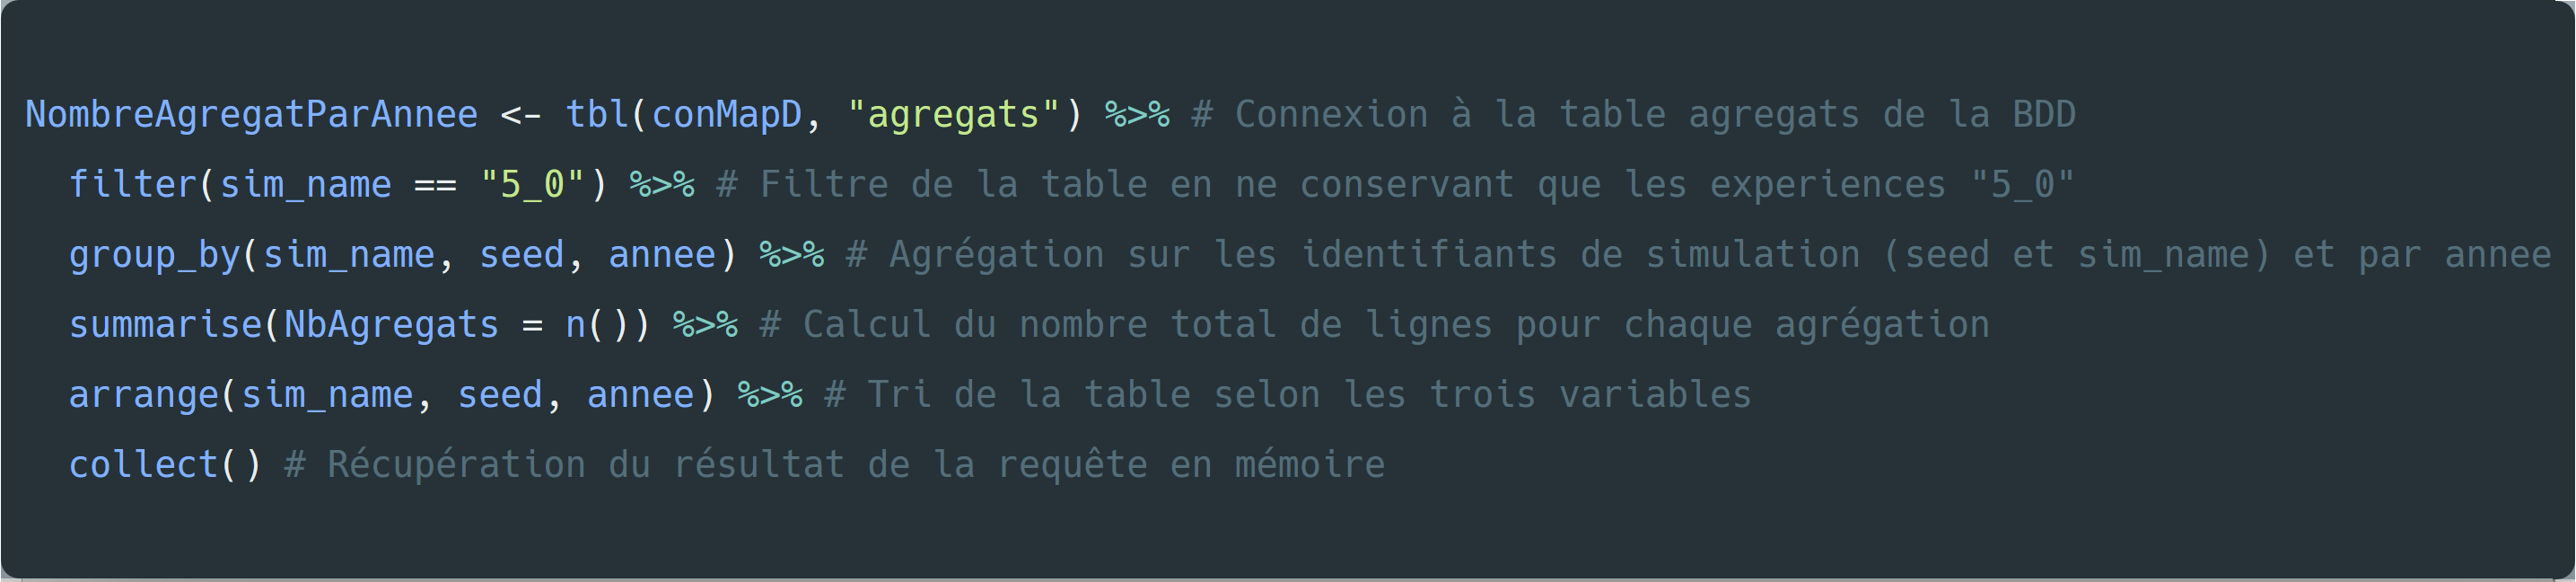
\includegraphics[width=\linewidth]{img/dplyr_cut.png}}
\vspace{-0.3cm}
\subfloat[Traduction du code source \textsf{dplyr} en \textsf{SQL}]{\label{subfig:exemple-dplyr-SQL}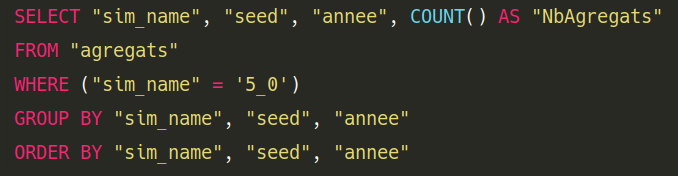
\includegraphics[scale=.35]{img/SQL_Sublime.png}}
\vspace{-0.3cm}
\caption{Un exemple de manipulation de données stockées dans un SGBD depuis \textsf{R}. On y interroge la table des agrégats de population pour calculer le nombre moyen d'agrégats par année de simulation.}
\label{fig:dml-simedb}
\end{figure}

\clearpage
\paragraph*{Création de graphiques avec \textsf{ggplot2} et la \og \textit{grammar of graphics}\fg{}}

\paragraph*{}
\begin{figure}[H]
\centering
\captionsetup{width=0.9\linewidth}
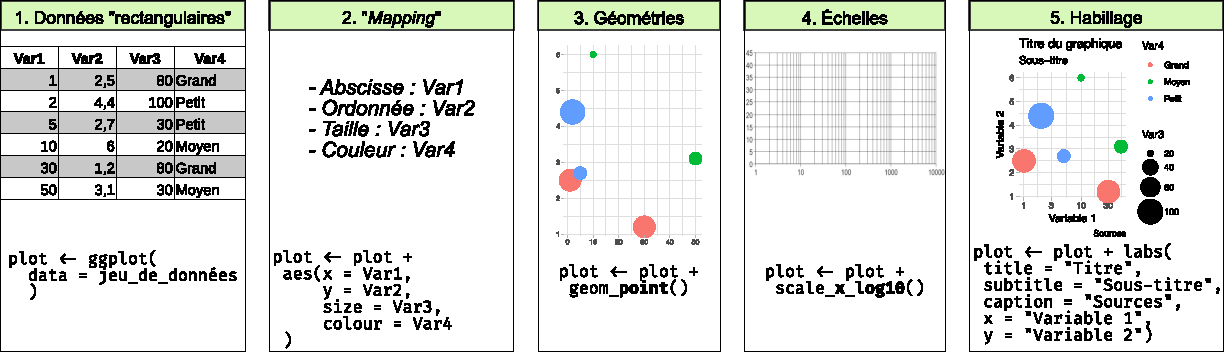
\includegraphics[width=\linewidth]{img/grammar-graphics-steps.pdf}
\caption{Représentation des éléments de grammaire de \textsf{ggplot2}, d'après une idée de \textcite{healy_data_2018}.
}
\label{fig:socviz-ggplot2}
\end{figure}


En interrogeant le SGBD avec des outils adaptés, on obtient un jeu de données qui servira de base à la représentation graphique des indicateurs (\cref{fig:socviz-ggplot2}, étape 1).
On peut passer alors passer à l'étape de construction graphique des indicateurs.
Il existe pour cela, toujours en restant de l'environnement (et du langage) \textsf{R}, de nombreux \textit{packages} dédiés.


L'un des \textit{packages} les plus utilisés, \textsf{ggplot2} \autocite{wickham_ggplot2_2016}, met en œuvre une syntaxe assez adaptée à nos contraintes : ce \textit{package} est conceptuellement fondé sur la \og \textit{grammar of graphics}\fg{}, c'est-à-dire une vision modulaire et très structurée de la conception graphique, pensée par Leland Wilkison \autocite{wilkinson_grammar_2006}.
La logique, assez familière pour un utilisateur de Systèmes d'Information Géographique (SIG), consiste à penser une représentation graphique comme un ensemble de couches (\textit{layers}), qui se superposent, se complètent, et sont toutes basées sur une source de données.
Les différentes composantes des données (variables par exemple) sont associées à des composantes graphiques de base (abscisse, ordonnée, taille, couleur \ldots), formant ainsi une mise en correspondance (\textit{mapping}) des données avec les composants graphiques (voir \cref{fig:socviz-ggplot2}, étape 2).

Dans notre cas, cette grammaire est porteuse d'un avantage majeur.
Elle est extrêmement structurée et modulaire.
Cela permet de ré-utiliser largement les codes-sources écrits pour un indicateur et de les adapter aisément à d'autres indicateurs.
Si la grammaire du graphique est bien définie, elle sera ainsi très indépendante du contenu des données que l'on y insère.


Par exemple, de nombreux indicateurs de sortie de SimFeodal décrivent l'évolution du nombre d'agents au cours des années de simulation (les agrégats dans la \cref{fig:exemple-ggplot2-simedb}).
Ce type de graphique est d'une part rapide à produire avec \textsf{ggplot2} : il ne requiert que quelques lignes de code (\cref{subfig:exemple-ggplot2-R}).
D'autre part, en changeant le tableau de données en entrée (créé dans \cref{subfig:exemple-dplyr-R}), on reproduit exactement le même type de graphique pour, par exemple, un autre type d'agent (le nombre de foyers paysans, d'églises\ldots).

Le \textit{package} \textsf{ggplot2} répond tout à fait aux contraintes de modularité exposées plus haut, et permet de factoriser le code-source, ce qui garantit une maintenance plus rapide et une meilleure robustesse de l'application dans son ensemble.


\begin{figure}[H]
\centering
\hspace{5pt}
\subfloat[Code source R avec le \textit{package} \textsf{ggplot2}]{\label{subfig:exemple-ggplot2-R}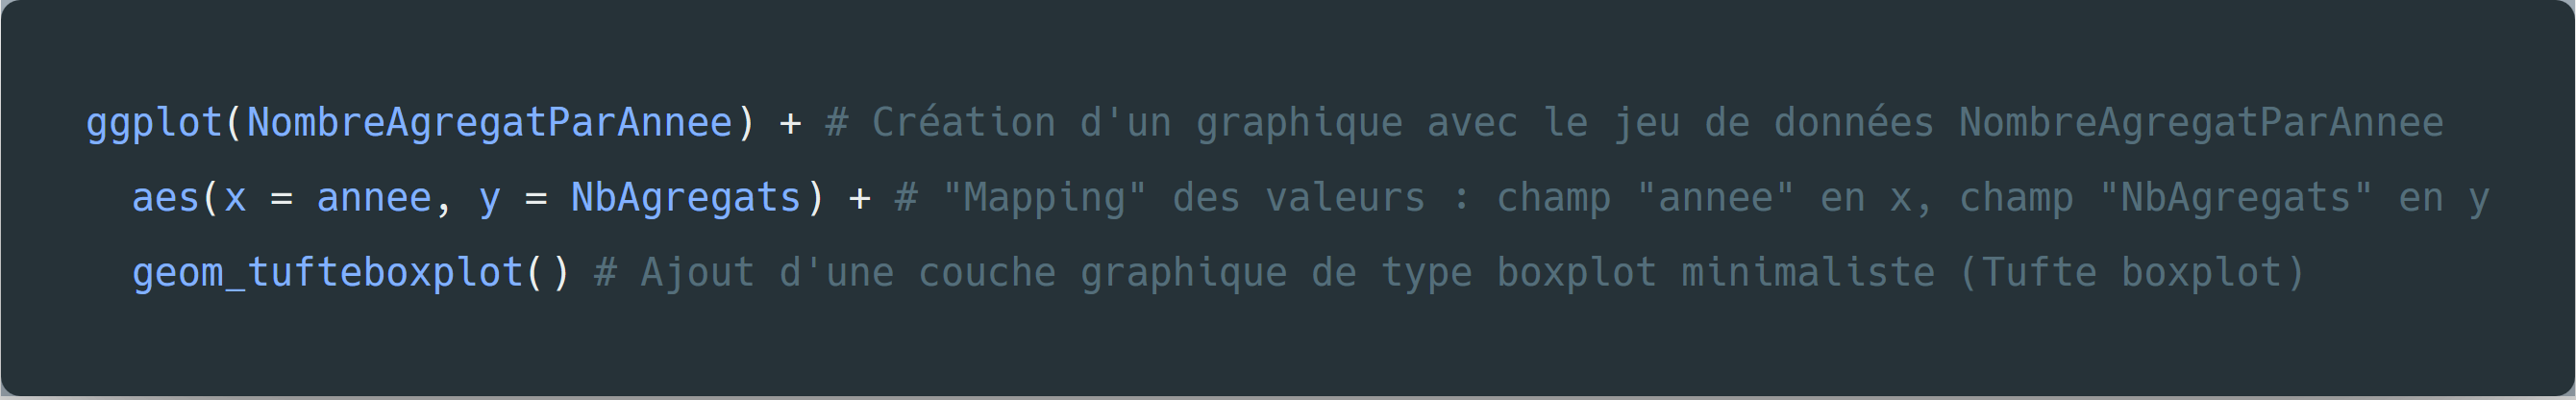
\includegraphics[scale=.15]{img/ggplot2.png}}
\hspace{5pt}
\subfloat[Graphique généré]{\label{subfig:exemple-ggplot2-plot}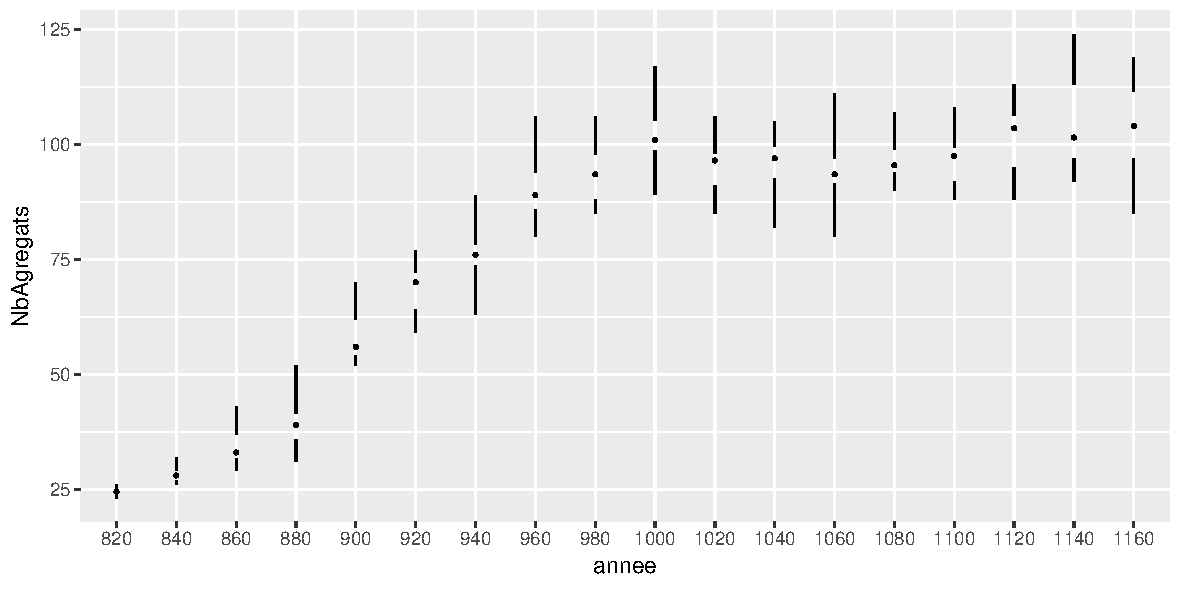
\includegraphics[width=\linewidth]{img/chap5_exemple_indicateur.pdf}}
\caption{Un exemple de manipulation de données stockées dans un SGBD depuis R.}
\label{fig:exemple-ggplot2-simedb}
\end{figure}

\paragraph*{Fluidifier les étapes de rendu : le \og pipeline de visualisation\fg{}}\label{par:visualisation-pipeline}

\textcite{dos_santos_gaining_2004} ont conceptualisé et schématisé l'ensemble des étapes nécessaires à la construction d'une visualisation, depuis les données brutes jusqu'à l'image finale, au sein d'un \og \textit{pipeline}\fg{} de la visualisation (\cref{fig:visualisation-pipeline}).
Ils y décrivent les différents états des données en entrée et en sortie (ligne supérieure), ainsi que les traitements que ces données subissent (ligne inférieure).

\begin{figure}[H]
	\centering
	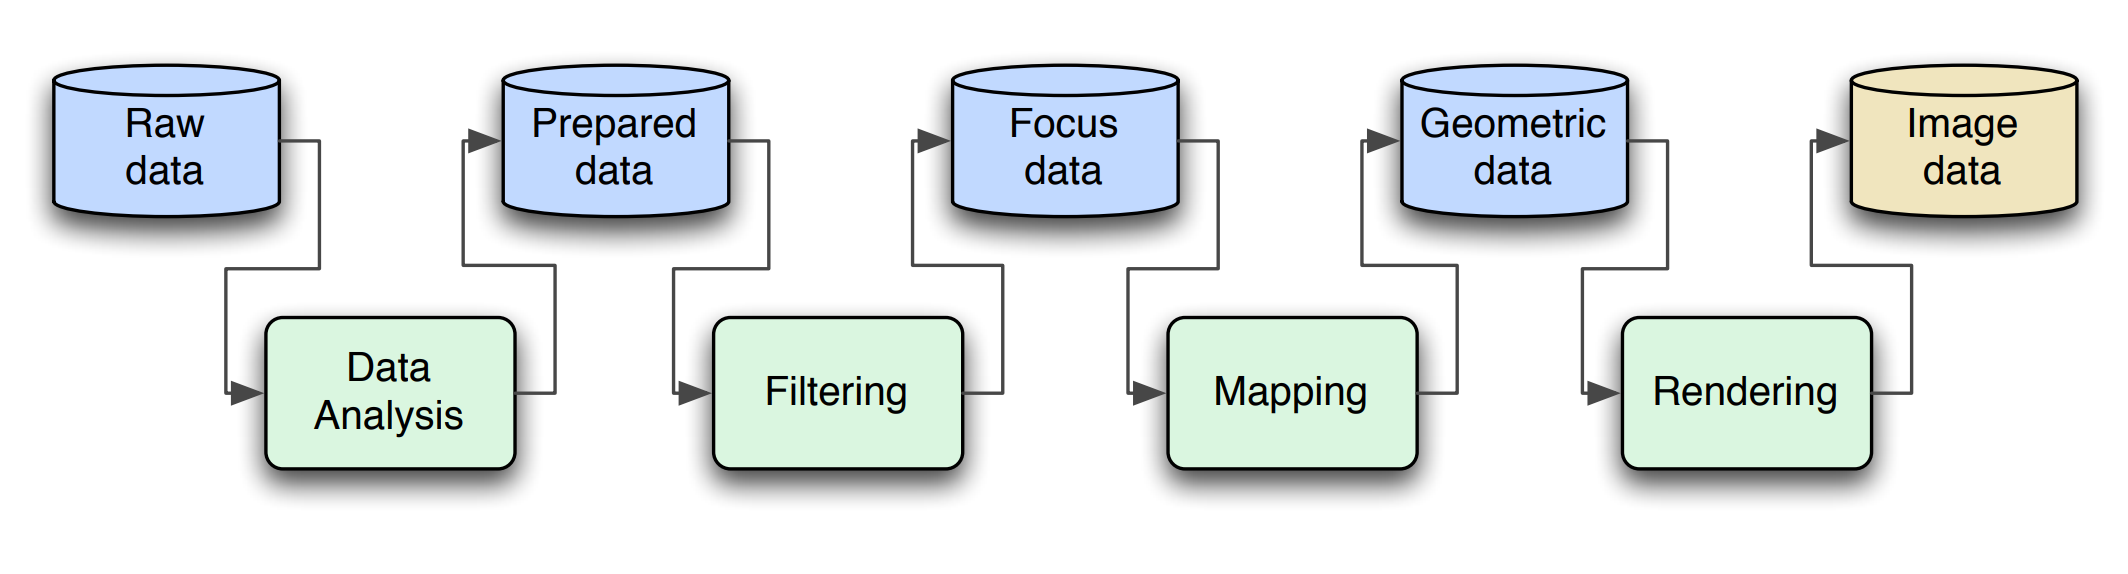
\includegraphics[width=\linewidth]{img/Visualisation_Pipeline_p92.png}
	\caption{\og \textit{The Visualisation Pipeline}\fg{}, de \textcite{keim_mastering_2010}, p.92, d'après \textcite{dos_santos_gaining_2004}, p. 314.}
	\label{fig:visualisation-pipeline}
\end{figure}

Ce \textit{pipeline} débute par des données brutes (\textit{raw data}) auxquelles ont fait subir un traitement (\textit{data analysis}, par exemple une agrégation) pour obtenir des données prêtes à l'utilisation (\textit{prepared data}).
Il s'agit ensuite de filtrer ces données (choix des expériences à conserver par exemple), dont l'on conserve donc uniquement les éléments nécessaires (\textit{focus data}).
Par une étape de mise en correspondance des variables et des primitives graphiques (\textit{mapping}, voir paragraphe précédent), on obtient un jeu de données \og géométriques \fg{} (\textit{geometric data}).
Cette \og géométrie\fg{} est à entendre au sens de l'espace de la représentation graphique, qui comprend par exemple les coordonnées des points, lignes, la couleur des cercles et autres éléments mobilisés dans la construction d'un graphique.
Il n'est donc aucunement question ici de données géographiques ou spatiales.
La dernière étape est plus technique : il s'agit du \og rendu graphique\fg{} (\textit{rendering}), qui convertit un ensemble de spécifications géométriques (textuelles) en une image affichable, faite de pixels (\textit{image data}).

Dans la chaîne de traitement la plus classique, ces étapes s'effectuent au sein de différents logiciels, chacun dédiés à une tâche. Dans le domaine des utilisateurs de SIG, on retrouve par exemple fréquemment une préparation des données dans un tableur, un import dans un logiciel SIG qui va être chargé de la cartographie, puis un export vers un logiciel de dessin vectoriel afin de réaliser la mise en page.
À chaque changement de logiciel, il est nécessaire d'exporter les données produites, puis de les ré-importer dans le logiciel suivant.

A contrario, le propre de l'utilisation d'un langage de programmation plutôt que d'un outil graphique est de pouvoir automatiser et intégrer l'ensemble de ces étapes.
L'utilisation de \textsf{R} comme langage de développement de SimEDB nous permet ainsi de développer une unique chaîne de traitement, qui ne requiert aucun import/export de données, et peut donc être consolidée, vérifiée et surtout ré-employée \textit{ad libitum}.

L'enchaînement des \textit{packages} employées dans SimEDB est présenté dans la \cref{subfig:visualisation-pipeline-simedb}, et le code-source correspondant à l'exemple développé dans cette sous-partie dans la \cref{fig:visualisation-pipeline-exemple}.

\begin{figure}[H]
\centering
\subfloat[Technologies utilisées dans SimEDB.]{\label{subfig:visualisation-pipeline-simedb}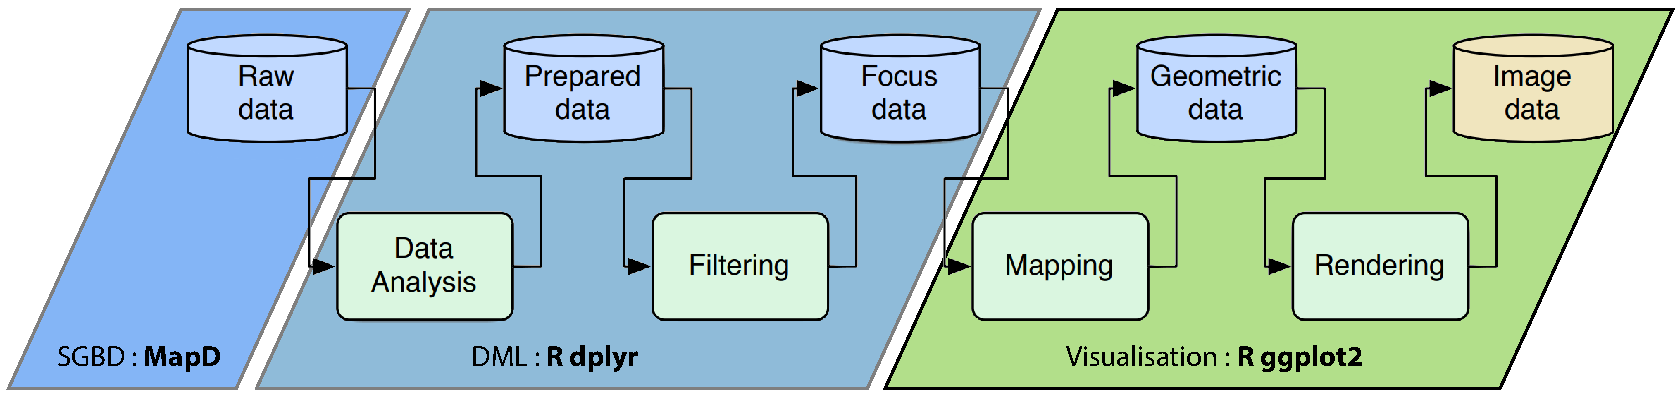
\includegraphics[width=\linewidth]{img/Visualisation_Pipeline_SimEDB.pdf}}
\hspace{5pt}
\subfloat[Implémentation d'un exemple de pipeline de visualisation pour construire un indicateur dans SimEDB]{\label{subfig:exemple-pipeline-simedb}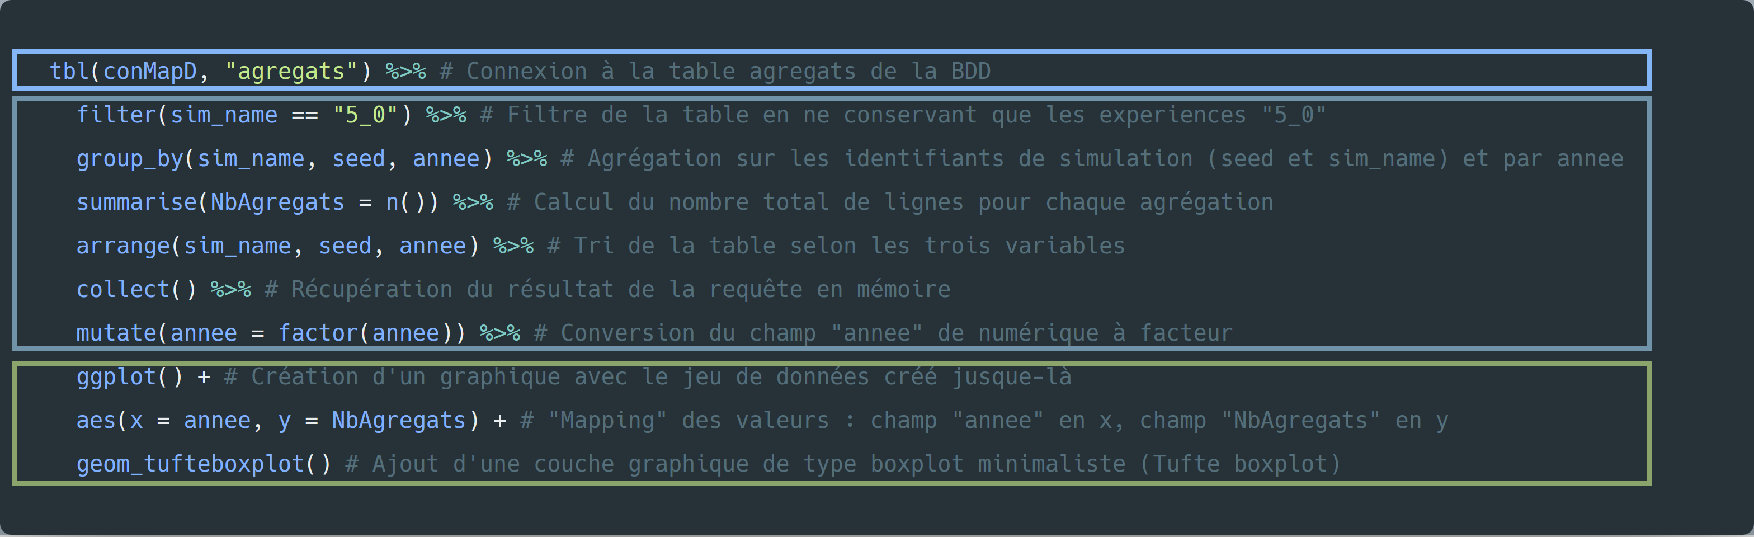
\includegraphics[width=\linewidth]{img/simedb_pipeline_R.pdf}}
\caption{Le \og pipeline\fg{} de visualisation et son implémentation dans SimEDB. Cette implémentation est obtenue en assemblant les codes des \cref{subfig:exemple-dplyr-R,subfig:exemple-ggplot2-R}.}
\label{fig:visualisation-pipeline-exemple}
\end{figure}

\paragraph*{Modulariser les fonctions}

\textsf{Shiny}, en tant qu'outil de création d'interface graphique, bénéficie aussi d'un avantage important en matière de conception d'application web : comme ce \textit{package} est basé sur un langage de programmation modulaire, on peut logiquement créer et ré-utiliser des \og briques d'interfaces\fg{} modulaires.
Par l'utilisation de modules\footnote{\href{https://shiny.rstudio.com/articles/modules.html}{https://shiny.rstudio.com/articles/modules.html}}, il est possible de définir un ensemble d'éléments graphiques adaptatifs et de ré-utiliser tel quel cet ensemble.

Dans l'interface de SimEDB (\cref{fig:simedb-modules}), par exemple, les indicateurs graphiques sont toujours présentés de la même manière (encadrés oranges) : dans la partie de droite relative aux indicateurs, l'indicateur à proprement parler est à gauche, et des outils de téléchargement (vectoriel et image) et de notation de l'indicateur (les étoiles) sont placés en haut à droite.

En termes de code-source, la manière de produire les deux indicateurs comparés dans la \cref{fig:simedb-modules} est strictement identique : c'est une fonction générique qui prend en entrée des données et un type de graphique à produire.
Dans la figure, seul un paramètre varie : le filtre appliqué aux données, qui renvoie ici à différentes expériences.
Cela permet donc d'une part de minimiser la taille du code, mais surtout, avec la généricité apportée, de faciliter de manière considérable l'ajout ou la modification d'indicateurs.

\begin{figure}[H]
\centering
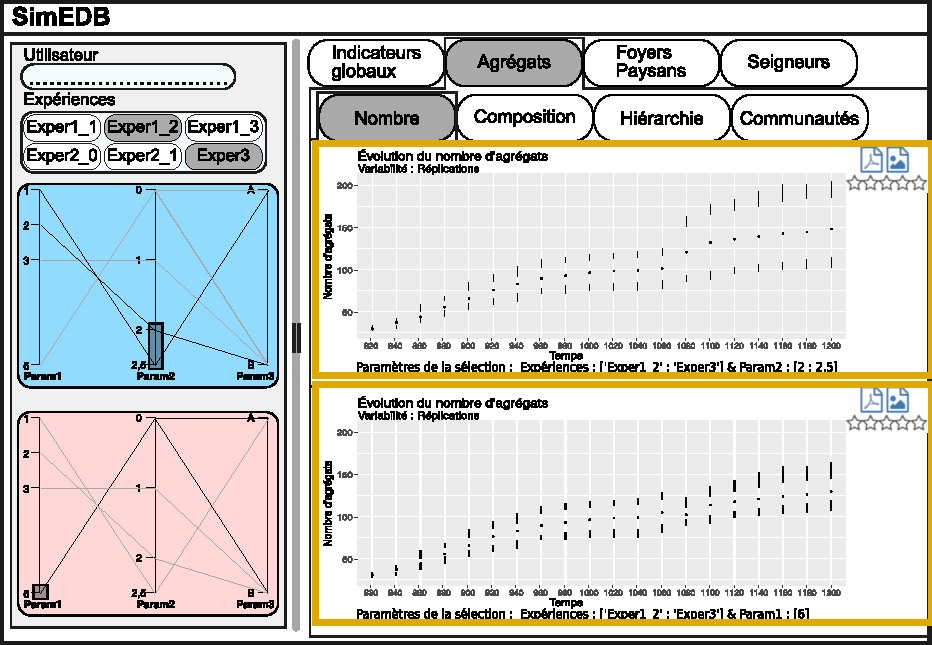
\includegraphics[width=\linewidth]{img/mockup_SimEDB_modules.pdf}
\caption{Une conception modulaire. Les deux éléments graphiques encadrés sont créés par un même \og module\fg{} dont les arguments varient.
Ici, l'argument est constitué par les expériences sélectionnées : on le visualise dans les graphiques en coordonnées parallèles (gauche) et dans la partie inférieure des des graphiques (texte \og Paramètres de la sélection\fg{}).\\
\textbf{N.B} : À partir de cette figure, on représente l'interface de SimEDB à l'aide d'un \textit{mockup} plutôt que de captures d'écrans, pour que les composants de l'interface soient plus facilement distinguables.}
\label{fig:simedb-modules}
\end{figure}


\subsubsection{Choix de l'organisation visuelle}

Les différentes étapes de construction d'une plate-forme d'exploration (\cref{sec:explorer-sorties-simfeodal} : \cnameref{sec:explorer-sorties-simfeodal}) ont conduit à une organisation sous forme de \textit{dashboard} interactif.
La forme de ce \textit{dashboard} a évolué tout au long de l'apparition de nouveaux besoins, pour aboutir sur une organisation mono-page, pensée autour de la consultation d'indicateurs de sorties, qui devaient permettre de comparer des expériences différentes sélectionnées au moyen de graphiques en coordonnées parallèles.

Le choix d'un outil dédié à la comparaison, plus qu'à la visualisation des résultats d'un unique ensemble de simulations, entraîne nécessairement des répercussions en matière de présentation visuelle -- d'interface graphique -- des éléments permettant de mener cette comparaison.
Depuis la première plate-forme aboutie -- SimVADB (\cref{fig:simvadb_dashboard}, reprise ici en \cref{subfig:mini-simdavb}) --, l'interface graphique a fortement évolué par conséquent (\cref{subfig:mini-simedb}).
\vspace{-0.25cm}
\begin{figure}[H]
	\centering
	\subfloat[SimVADB]{\label{subfig:mini-simdavb}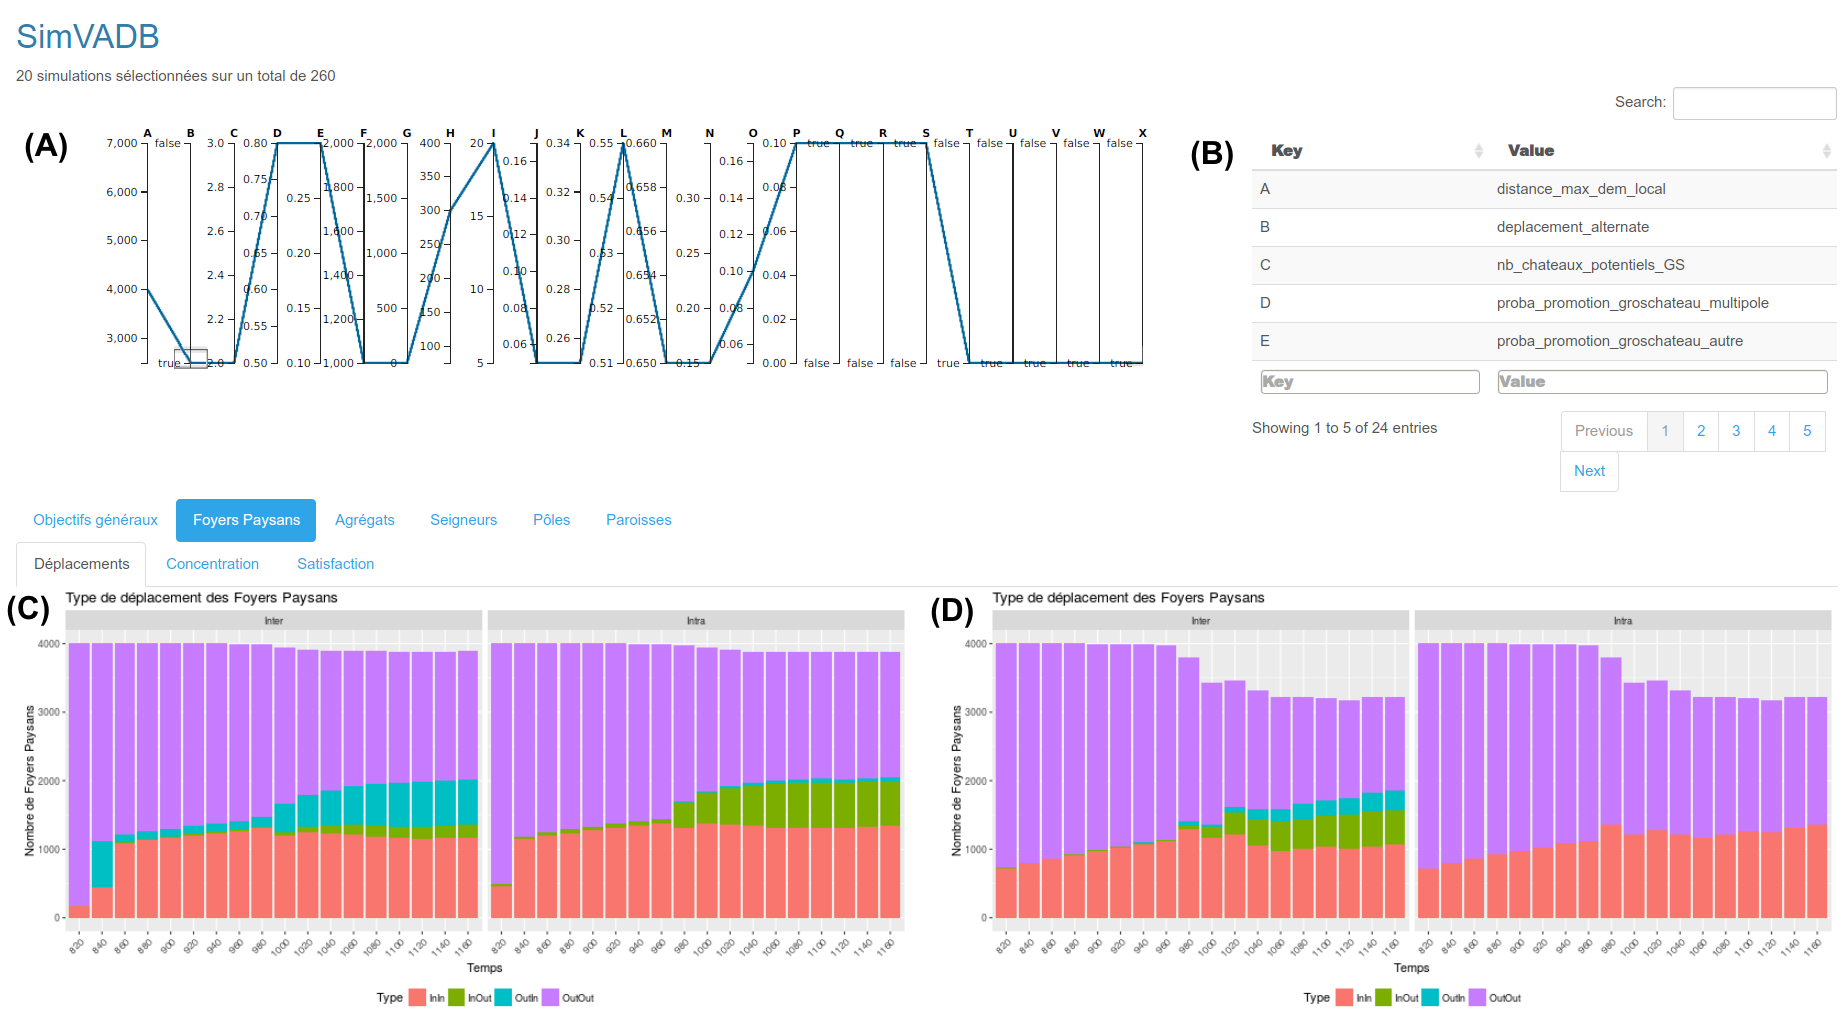
\includegraphics[width=.9\linewidth]{img/SimVADB_Dashboard2_annote_retouche.png}}\\[-1.5ex]
	\hspace{1pt}
	\subfloat[SimEDB]{\label{subfig:mini-simedb}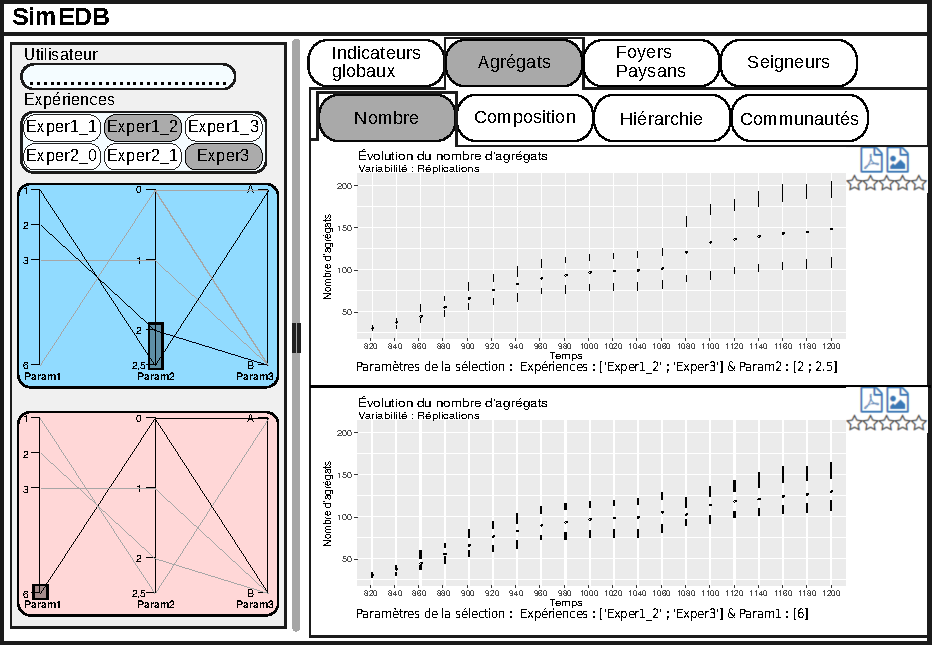
\includegraphics[width=.9\linewidth]{img/mockup_SimEDB.pdf}}
	\vspace{-0.3cm}
	\caption{Comparaison visuelle de SimVADB (a) et SimEDB (b).}
	\label{fig:comparaison-simvadb-simedb}
\end{figure}


\paragraph*{Une comparaison verticale}

Le premier changement tient à la disposition des \og contrôleurs\fg{}, c'est-à-dire aux composants de l'interface sur lesquels l'utilisateur peut jouer pour choisir les expériences qui seront affichées.
Dans SimVADB, le seul contrôleur était un graphique en coordonnées parallèles interactif, situé dans le haut à gauche de l'interface (\cref{subfig:mini-simdavb}, partie \textbf{(A)}).
Celui-ci permettait de régler le choix des expériences présentées dans l'indicateur de droite (\textbf{D}), celui de gauche (\textbf{C}) étant constitué d'une moyenne de l'ensemble des expériences.

Dans SimEDB, on a déjà expliqué le choix de permettre une double sélection, c'est-à-dire de régler les deux sous-ensembles de simulation à comparer.
Par conséquent, la barre des contrôleurs (encadré orange dans la \cref{fig:simedb-sidebar}) est désormais constitué de deux graphiques en coordonnées parallèles interactifs (en bleu et en rouge), qui agissent sur les indicateurs présentés à leur droite.

\begin{figure}[H]
	\centering
	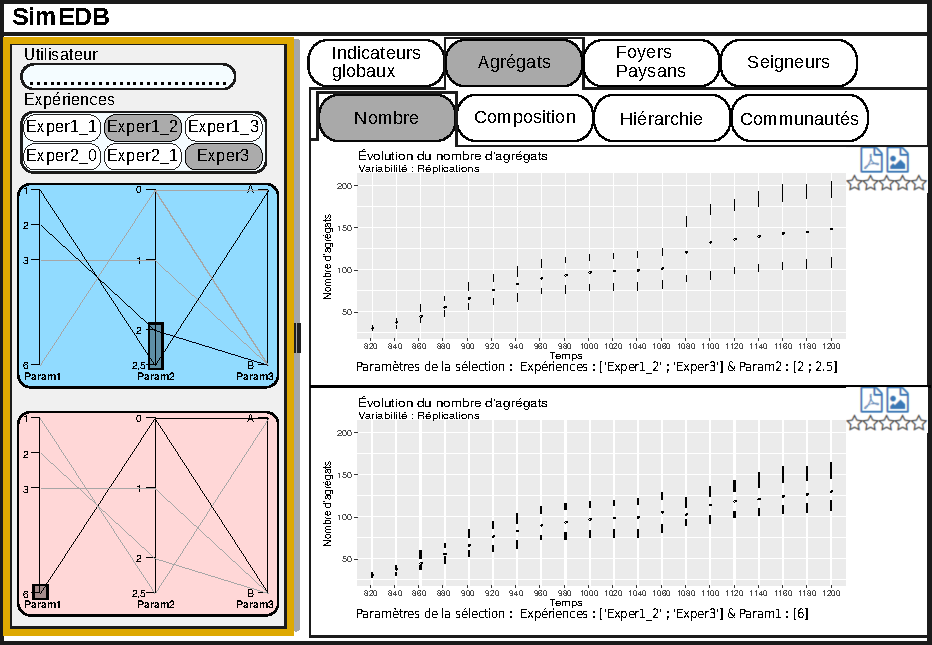
\includegraphics[width=\linewidth]{img/mockup_SimEDB_controleurs.pdf}
	\caption{La barre de contrôleurs (encadrée en orange) dans l'interface de SimEDB.}
	\label{fig:simedb-sidebar}
\end{figure}

En raison de ces composants supplémentaires dans l'interface, on a choisi d'en changer la disposition. Les contrôleurs sont désormais situés à gauche et les indicateurs à droite, alors qu'ils étaient superposés dans SimVADB.

Ce choix de re-disposition tient à deux arguments.
En premier lieu, en termes d'occupation de l'espace visuel on peut noter que les indicateurs graphiques sont toujours plus larges que haut.
Cela s'explique notamment de manière thématique, en ce que la variation temporelle, souvent présentée en abscisse, est plus importante que les valeurs attributaires, en ordonnée : les indicateurs de ce type s'analyse plus de manière relative, en observant leur évolution, que de manière absolue.
L'occupation de l'espace visuel est donc mieux employée en superposant les indicateurs : cela permet d'augmenter la taille de chacun.

La seconde raison est méthodologique.
SimEDB est un outil qui sert à comparer visuellement des données de sortie de simulation.
Dans les indicateur présentés, le plus souvent, les intervalles affichés en abcisse sont constants : qu'ils s'agissent du temps, de modalités d'un indicateur (petits seigneurs, grands seigneurs\ldots) ou encore de seuils (composition d'un agrégat en nombre de foyers paysans, discrétisée selon des seuils choisis en amont), l'axe des abscisse est identique quelles que soient les expériences comparées.
L'axe des ordonnées, au contraire, est plus variable : qu'il représente une valeur absolue, un décompte ou une fréquence, les ordres de grandeur de ces valeurs sont très hétérogènes selon les expériences comparées.
Le choix a donc été fait de présenter visuellement les ordres de grandeur comparables, et donc de superposer les sélections différentes (l'axe des abscisses est alors commun) plutôt que de les afficher côte-à-côte (ce qui aurait complexifié la comparaison des ordonnées en les présentant comme directement comparables alors que les ordres de grandeur varient).


Avec un axe \og fixe\fg{}, il est donc opportun de mener la comparaison visuelle sur cet axe, et donc d'aligner les graphiques sur celui-ci. L'organisation des différents indicateurs est donc verticale plutôt qu'horizontale.
Afin que la sélection des simulations à explorer soit intuitive, les contrôleurs doivent être alignés aux indicateurs, et dès lors, verticalisés eux aussi.
Pour bien différencier visuellement ce qui relève d'un affichage et ce qui requiert une interaction, les contrôleurs s'inscrivent dans un panneau dédié, grisé (\cref{fig:simedb-sidebar}), ce qui constitue presque un standard dans les interfaces modernes d'applications interactives.

\paragraph*{Onglets et sous-onglets}

Comme dans SimVADB (\cref{subfig:mini-simdavb}), on a choisi de conserver une navigation entre indicateurs par un systèmes d'onglets imbriqués : un premier niveau d'onglets permet d'accéder au type d'agents concernés par les indicateurs, et un second niveau permet de sélectionner spécifiquement l'indicateur choisi\footnote{
Notons que cette question revêt une importance réelle en matière d'ergonomie de l'application, mais que l'aspect technique en est pourtant assez simple.
Pour changer le mode d'organisation des onglets et sous-onglets, il suffirait de ré-organiser les appels aux composants dans le code-source de l'application.
}.

En terme de disposition, cela force l'utilisateur à interagir avec l'application régulièrement puisque chaque indicateur doit être sur un onglet dédié.
La majorité des utilisateurs potentiels de SimEDB consultent toutefois l'application sur des ordinateurs portables, dotés d'écran réduits et d'une résolution faible.
L'encombrement visuel est alors atteint rapidement, et mieux vaut présenter un indicateur à la fois plutôt que de présenter l'ensemble des indicateurs sur une unique page : la démarche d'étude visuelle sera plus longue, mais ne sera pas gênée ou faussée par des graphiques de dimension trop réduites qui peuvent induire des erreurs de lecture.

%On aurait pu privilégier une vision globale, par exemple en affichant d'un coup, pour chaque type d'agents, l'ensemble des indicateurs concernés.
%Sur des écrans de grande dimension, cela aurait permis d'embrasser du regard les résultats propres à chaque type d'agent bien plus rapidement, et d'accélérer d'autant l'évaluation de simulations ou leur comparaison.

L'organisation des onglets en eux-mêmes pose aussi une question importante : vaut-il mieux organiser la consultation par type d'agent, ou plutôt, hiérarchiquement, selon la catégorie de processus examinée (\hl{à corriger une fois fixé sur le terme}, \hl{faire ref au chap3}), par exemple en respectant l'ordre de consultation des indicateurs déterminé ?

Les deux approches présentent des avantages, mais nous avons choisi de rendre l'utilisation de SimEDB plus intuitive à tous, c'est-à-dire en organisant les indicateurs par type d'agents, plutôt qu'efficace, pour les utilisateurs habitués qui auraient bénéficié d'une organisation structurée hiérarchiquement.

\subsubsection{Choix des modes d'interactions}

Avant même la conception de SimEDB, avec la plate-forme SimVADB, nous avions décidé de baser la sélection des simulations sur des graphiques en coordonnées parallèles interactifs (\cref{subsec:explo-interactive} : \og \cnameref{subsec:explo-interactive}\fg{}).
La logique d'ensemble du filtrage de simulations restant la même, il n'était pas nécessaire de modifier ce choix pour SimEDB.

L'accumulation d'expériences, reposant sur les variations de paramètres différents, ainsi que la démultiplication des paramètres du modèle SimFeodal ayant accompagné son paramétrage, ont pourtant demandé de reconsidérer l'usage de ces graphiques interactifs.
Là où seuls quelques paramètres étaient mobilisés auparavant, les graphiques en coordonnées parallèles reposaient sur peu d'axes.
Avec l'augmentation du nombre d'axes, le graphique en coordonnées parallèle est rapidement devenu illisible faute à une surcharge graphique due au recouvrement des axes.

\paragraph*{Réduire la surcharge visuelle des graphiques en coordonnées parallèles}

La première mesure pour y remédier a été de filtrer les paramètres affichés : nul besoin d'afficher un axe correspondant à un paramètre qui n'est jamais manipulé dans les expériences.
Plutôt que de définir les paramètres \og utiles\fg{}, et donc d'avoir à les redéfinir dans l'application à chaque ajout d'expérience qui reposerait sur la variation d'un paramètre différent, nous avons fait en sorte que cette discrimination des paramètres \og actifs\fg{} soit exécutée de manière automatique :
quand SimEDB est lancé, une requête est exécutée sur la table des paramètres pour identifier ceux qui présentent plusieurs modalités et ceux qui n'en ont qu'une.
Seuls sont alors affichés les paramètres de la première catégorie, car eux-seuls présent un intérêt à être discriminés.

Ce faisant, le nombre de paramètre affichés est réduit, et permet d'afficher leurs intitulés plutôt que de faire appel à une table de correspondance comme dans SimVADB (\cref{subfig:mini-simdavb}, partie \textbf{(B)}).
L'automatisation de ce traitement permet de plus de ne pas avoir à changer quoi que ce soit à la plate-forme lors d'ajouts ou de suppressions de simulations de la base de données, ce qui concoure à l'objectif d'indépendance aux données de la plate-forme d'exploration.

\paragraph*{Pré-filtrer les simulations}

Au fur et à mesure du paramétrage puis de la calibration de SimFeodal, les expériences ont tout de même continué à mobiliser de plus en plus de paramètres différents.
Pour réduire la quantité d'information représentée et améliorer en conséquence \og l'expérience utilisateur\fg{}, nous avons ajouté un filtre, moins visuel que les graphiques en coordonnées parallèle, qui permet toutefois de restreindre le nombre de simulations affichées à partir de leur dénomination.
Plutôt que de cibler des valeurs spécifiques de paramètres, l'idée est donc de soustraire des choix possibles des expériences entières.
Pour SimEDB, on a donc ajouté un pré-filtrage, sous forme de \og boîte de sélection\fg{} (\textit{select input}, \cref{fig:simedb-prefilter}), qui interroge la base de données directement pour connaître les différents intitulés de simulations et agit comme un premier filtre réduisant donc les simulations interrogées dans les graphiques en coordonnées parallèles.

\begin{figure}[H]
\centering
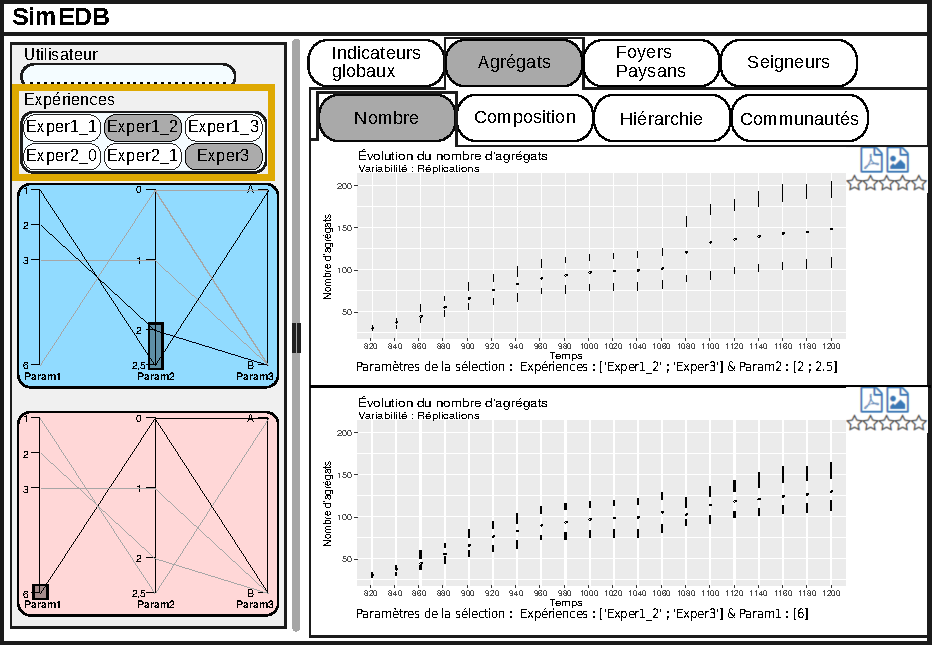
\includegraphics[width=\linewidth]{img/mockup_SimEDB_selectinput.pdf}
\caption{Le menu de sélection des expériences (encadré en orange) qui permet un pré-filtrage des expériences à partir de leur nom.}
\label{fig:simedb-prefilter}
\end{figure}

\paragraph*{Optimiser l'occupation de l'espace visuel}\label{par:simedb-resize-parcoords}

En dépit de ces différentes techniques visant à minimiser le nombre d'axes affichées dans les graphiques en coordonnées parallèles, la place prise par ces graphiques reste importante, en particulier quand on décide de ne pas diminuer la taille des éléments de légende afin de conserver leur lisibilité.
Quand l'application est consultée sur un écran de taille faible, l'appréhension de l'ensemble des informations présentes dans l'interface pose ainsi un véritable problème.

En réfléchissant aux séquences d'usages, par les utilisateurs, de SimEDB, on a pu comprendre que le mode d'utilisation le plus classique était de bien considérer le filtrage à effectuer sur les graphiques en coordonnées parallèles, en y consacrant un temps certain, avant de comparer longuement les différents indicateurs de la sélection.
Il n'est donc que rarement fait usage de multiples filtres successifs sur un seul indicateur, dans une approche plus exploratoire donc, mais plutôt d'évaluations complètes de simulations choisies.

Il n'est alors plus indispensable de consacrer une part importante de l'espace aux zones interactives (le panneau de contrôle), ou du moins, pas pendant l'ensemble de la période d'évaluation des simulations.

Un outil de redimensionnement a alors été ajouté à SimEDB, permettant, par glisser-déposer, de modifier la largeur occupée par le panneau de contrôle en l'adaptant à chaque moment au besoin de visualisation.
La \cref{fig:resizing} montre ainsi une succession d'états : en début d'exploration, l'utilisateur va augmenter la taille du panneau de contrôle pour augmenter la lisibilité des graphiques en coordonnées parallèles et effectuer une sélection plus simplement.
Une fois la sélection effectuée, il pourra alors re-diminuer la largeur du panneau afin d'augmenter la zone disponible pour les indicateurs de sorties de simulation, et donc la taille de ces derniers. 

\begin{figure}[H]
\centering
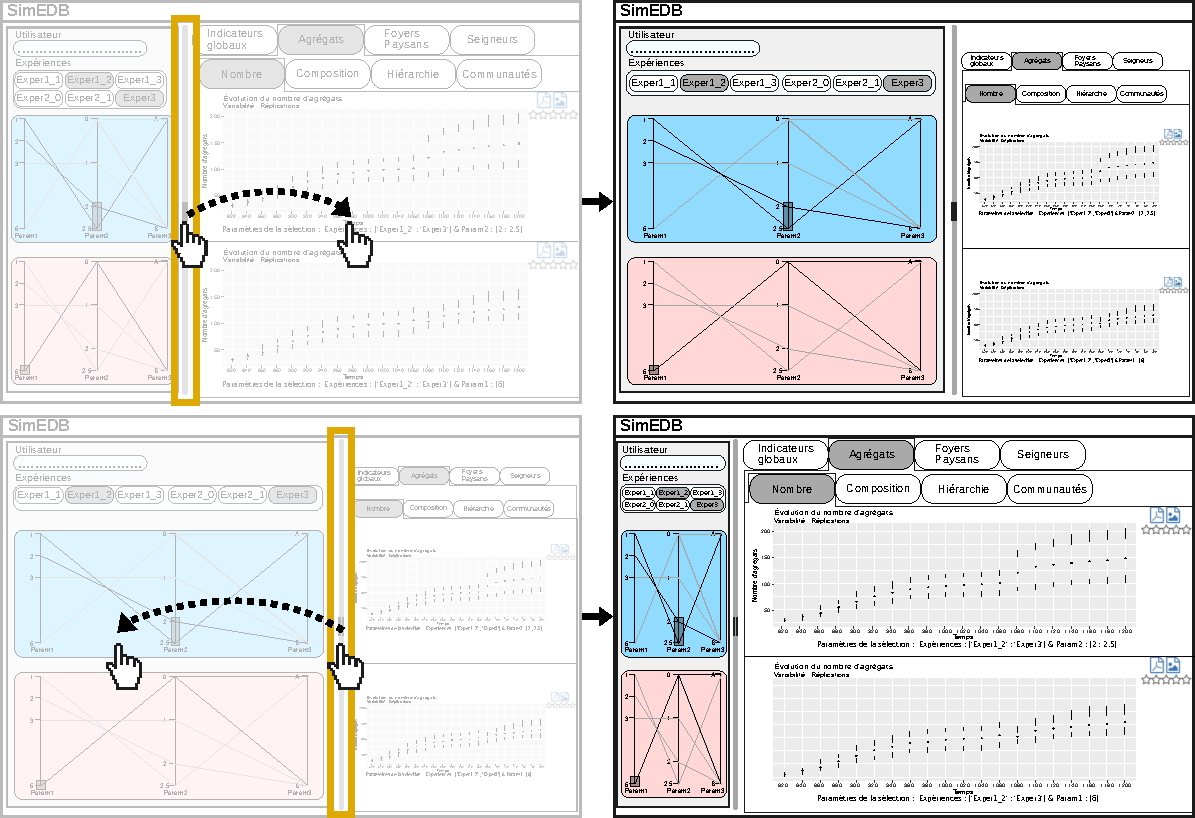
\includegraphics[width=\linewidth]{img/mockup_SimEDB_resize.pdf}
\caption{Utilisation interactive de SimEDB et redimensionnement du panneau de contrôle.}
\label{fig:resizing}
\end{figure}

\paragraph*{Répondre aux demandes des utilisateurs : ajout d'un mécanisme d'export des indicateurs}

L'intérêt d'une interface modulaire et factorisée se révèle véritablement quand les utilisateurs d'un outil demandent des fonctionnalités supplémentaires, non prévues lors de la conception de l'outil.
Dans le cas de SimFeodal, une telle requête est rapidement apparue : les thématiciens, mais aussi les modélisateurs, pour conserver une trace d'une session d'exploration des indicateurs, souhaitaient pouvoir exporter les graphiques correspondant aux indicateurs.

Si au départ, une simple capture d'écran pouvait suffire, ce besoin a été complété par une volonté d'inclure des indicateurs de simulations dans des articles et autres communications, requérant donc des retouches des graphiques.
Pour ce faire, on a choisi d'ajouter des fonctionnalités de téléchargement des graphiques, selon deux formats -- image et vectoriel -- afin de satisfaire à ces deux usages.
Avec le développement modulaire adopté, il a suffit d'ajouter ces fonctions d'export en un unique lieu dans le code-source de SimEDB, et l'ajout de ces nouvelles fonctionnalités a alors été disponible automatiquement pour chacun des indicateurs graphiques.

Un autre élément répond à une demande forte des utilisateurs : dans une ré-utilisation hors application des indicateurs, il était difficile de se souvenir des sélections effectuées pour produire un indicateur : en terme de reproductibilité, une fois un graphique exporté sur un ordinateur, il n'y avait plus aucun moyen de connaître les conditions précises de sa création.
Nous avons donc ajouté, sur les graphiques eux-mêmes, un résumé des expériences et valeurs de paramètres sélectionnées dans chacun des indicateurs.
Cela permet d'en conserver une trace plus durable et augmente leur potentiel réutilisation.

\paragraph*{Noter les simulations}

Un dernier point d'interaction avec l'application a été prévu, sans pouvoir toutefois être mobilisé jusque là : il s'agissait d'aller vers une semi-automatisation de l'évaluation des simulations, par l'intermédiaire d'un outil graphique permettant de \og noter\fg{} les simulations sélectionnées.
Pour ce faire, et parce que, on l'a vu, l'évaluation d'un ensemble de simulations ne peut se faire de manière unique, on a choisi de donner la possibilité aux utilisateurs experts de noter chacun des indicateurs de sortie, pour chacun des ensembles de simulations qu'ils exploreraient.
L'évaluation se fait au moyen d'un outil simple, composé de 5 \og étoiles\fg{}, et est enregistré à chaque nouvelle note.

Une piste d'utilisation serait de mobiliser les données ainsi créées, composées d'une note donnée à un indicateur pour un ensemble d'identifiants uniques de simulations, afin de réaliser des analyses quantitatives des notes attribuées : est-ce que certaines simulations sont systématiquement bien notées avec chacun des indicateurs affichés ? Certains indicateurs ne sont-ils jamais observés ou ne donnent-ils jamais lieu à évaluation ?

Cette fonctionnalité, bien qu'implémentée, n'est pas encore utilisée, mais devrait à terme permettre d'aller vers une meilleure connaissance des résultats de simulation, tout autant que vers une mesure de l'efficacité des indicateurs de sortie choisis pour évaluer un ensemble de simulations.

\subsubsection{Présentation générale}

SimEDB est une application interactive.
Il nous semblait dommage d'en présenter l'utilisation d'ensemble par une succession de captures d'écran commentées.
Nous avons donc réalisé une vidéo qui en montre l'usage et est disponible à cette adresse : \hl{A faire...}
